\documentclass{elteikthesis}

% Overleaf: keep this file named main.tex and select pdfLaTeX in Project Settings.
% Local build: make  (or: latexmk -pdf main.tex)
% -----------------------------------------------------------------------------
% Student metadata -- must match the approved topic registration exactly.
% -----------------------------------------------------------------------------
\title{AI-Assisted Discovery of Dynamic Graph Algorithms via Evolutionary Code Repair}
\author{Thonmay Md Thoriqul Islam}
\neptun{FFR8A9}
\degree{Computer Science BSc}
\date{2026}

% Copy supervisor and programme metadata exactly from the approved topic form.
\supervisor{Gregory Reynolds Morse}
\affiliation{Lecturer and MSc in Computer Science}

\university{Eötvös Loránd University}
\faculty{Faculty of Informatics}
\department{Department of Programming Languages and Compilers}
\city{Budapest}
\logo{elte_cimer_szines}

% Draft mode displays structural advice in grey. Set false before submission.
\newif\ifshowtemplateguidance
\showtemplateguidancetrue

% Optional convenience packages may be added here. Avoid minted unless the
% project deliberately enables shell escape; listings works without it.

\newcommand{\TemplateGuidance}[1]{%
  \ifshowtemplateguidance
    \begin{quote}\small\color{gray!80!black}
      \textbf{Template guidance --- remove for submission.} #1
    \end{quote}
  \fi
}

\newcommand{\TemplatePrompt}[1]{%
  \ifshowtemplateguidance
    \par\noindent\textcolor{gray!80!black}{\textit{#1}}\par
  \fi
}

\newcommand{\MissingArtifactPage}[2]{%
  \clearpage
  \thispagestyle{empty}
  \begin{center}
    \vspace*{35mm}
    {\Huge\bfseries\textcolor{red!70!black}{MISSING REQUIRED ARTIFACT}}\\[12mm]
    {\Large\bfseries #1}\\[12mm]
    \begin{minipage}{0.75\textwidth}\centering #2\end{minipage}
  \end{center}
  \clearpage
}

\newcommand{\EvidenceTable}{%
  \begin{table}[H]
    \centering
    \caption{Contribution-to-evidence map; replace every placeholder.}
    \label{tab:contribution-evidence}
    \begin{tabularx}{\textwidth}{@{}p{0.18\textwidth}X X@{}}
      \toprule
      \textbf{Contribution} & \textbf{What is original or difficult} & \textbf{Where it is proved} \\
      \midrule
      C1 & <precise contribution> & <requirements, design, code, tests, results> \\
      C2 & <precise contribution> & <requirements, design, code, tests, results> \\
      C3 & <precise contribution> & <requirements, design, code, tests, results> \\
      \bottomrule
    \end{tabularx}
  \end{table}
}


\begin{document}
\documentlang{english}

\hypersetup{pageanchor=false}
\maketitle
\pagenumbering{gobble}

% Export the approved registration form to this exact filename.
\IfFileExists{approved-topic-registration.pdf}{%
  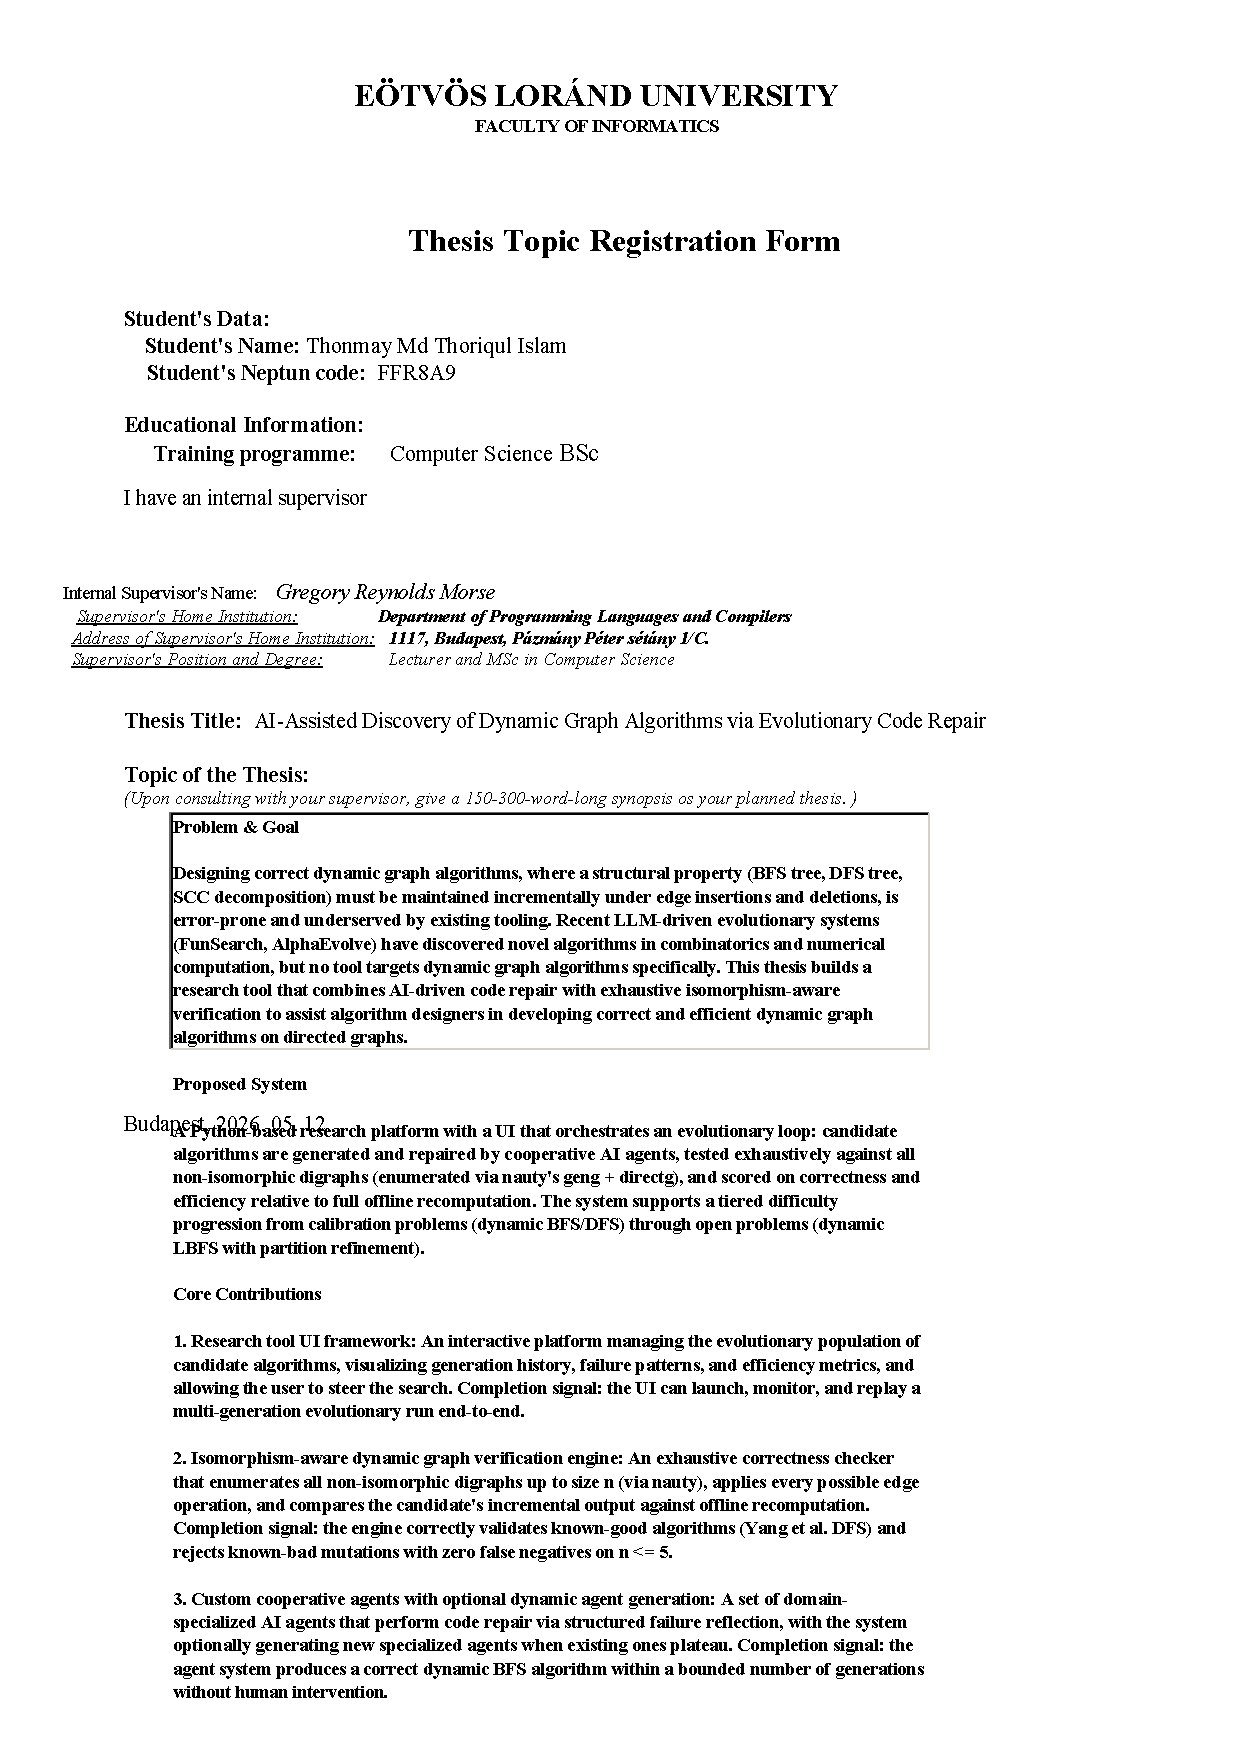
\includepdf[pages=-,pagecommand={\thispagestyle{empty}}]{approved-topic-registration.pdf}
}{%
  \MissingArtifactPage{Approved Topic Registration Form}{%
    Export the approved form as \texttt{approved-topic-registration.pdf} and upload it
    beside \texttt{main.tex}. Confirm the exact current submission package with ELTE IK.}
}

\cleardoublepage
\hypersetup{pageanchor=true}
\pagenumbering{arabic}
\setcounter{page}{1}
\tableofcontents

\chapter{Introduction}
\label{ch:introduction}

\section{Motivation and problem}
\label{sec:motivation}

The topic came out of a discussion with my supervisor, Gregory Morse, before the
thesis registration. I was already working with AI agents during my internship
at Ericsson, and he suggested a topic in which agents would be used to discover
algorithms. After going through a few options I chose this one, because it
builds on what I do at work and takes it further: instead of using agents to
write ordinary code, the goal is to use them to find algorithms that are both
correct and efficient.

The problem is keeping a graph search structure up to date while the graph
changes. When an edge is inserted or deleted, a dynamic algorithm has to update
a BFS tree, a DFS tree or an LBFS ordering without recomputing it from scratch.
The idea is simple, but the details are easy to get wrong. Each structure has
invariants that must hold after every update: the BFS distances must agree with
the parent pointers, the DFS discover and finish times must nest properly, and
the LBFS ordering must keep its four-point property. One stale value or one
wrong tie-break is enough to break them. The known correct algorithms
\citep{demetrescu2005dynamic,even1981maintaining,friglioni2000,
yang2019dynamic,baswana2019dynamic,baswana2017,corneil2008unified} are
complicated enough that they are usually proved correct rather than tested.

I chose BFS, DFS and LBFS because they are the basic graph searches that many
other algorithms build on: BFS for shortest paths and layering, DFS for cycle
and connectivity tests, and LBFS for chordal-graph recognition and maximum
cardinality search \citep{morse2026bfs,brandstadt1997lexbfs,habib2000lexbfs,
berry2004mcs}. They also give a natural difficulty scale. Correct dynamic BFS
and DFS algorithms are already known \citep{yang2019dynamic,morse2026bfs}, so
they show whether the tool works at all; dynamic LBFS has been studied much
less, so it is the harder test. During development, the first problem I tried
was dynamic MCS, as a smaller starting point, before moving to these three.

Language models can now write and fix code \citep{chen2021codex,openai2025codex,
jimenez2024swebench}, and systems such as FunSearch and AlphaEvolve pair a model
with an evolutionary loop and have found new algorithms and mathematical
constructions \citep{funsearch2023,alphaevolve2025,alphatensor2022,lehman2023elm}.
The repair side has a longer history in genetic programming and automatic
program repair \citep{koza1992gp,legoues2012genprog}, and more recently in
agents that reflect on their own failures \citep{reflexion2023,
madaan2023selfrefine,yao2023react}. All of these systems judge a candidate by
running it on test inputs. For a dynamic graph algorithm that is not enough: a
candidate can pass every test and still fail on a small graph with one
particular order of updates \citep{claessen2000quickcheck,jia2011mutation}. I
saw this in my own evaluation. One candidate passed every graph up to four
vertices and failed 1 of 51{,}465 cases at five, and one of the seven one-line
mutations of the fully dynamic DFS of \citet{yang2019dynamic} fails only after
several updates, never after a single one (Section~\ref{sec:test-selftest}).

So I wanted a tool in which the agents and the checking are designed together.
Instead of testing on examples, the verifier checks a candidate on every graph
up to a size bound (one per isomorphism class), and the agents get the failing
case back as feedback. The tool can also be driven by an external coding agent,
not only by its own agents. To my knowledge, no existing tool does this for
dynamic graph algorithms. Within the stated bound, the tool reports that no
counterexample was found, and I use it to search for, verify and measure dynamic
BFS, DFS and LBFS algorithms, reporting both positive and negative results.

\section{Goal, scope, and success criteria}

The goal is a research tool that helps an algorithm designer develop a correct
and efficient dynamic graph algorithm: a Python package with a command line, a
local web interface and a harness mode for external coding agents, with an
experimental evaluation on a tiered set of problems.

The scope is a tiered problem set. Dynamic BFS and dynamic DFS form the
calibration tier, where a correct algorithm is known to be reachable, and
dynamic LBFS forms the open tier, where the search is not guaranteed to succeed.
The problems are directed except LBFS, which is undirected. The tiering is what
makes the evaluation interpretable: the calibration tier measures whether the
tool can find and verify a correct algorithm at all, and the open tier measures
whether it can do so on a problem where success is not assumed.

Two boundaries are stated explicitly as non-goals. First, verification is
bounded: a passing candidate has no counterexample within the stated graph-size
and sequence bound, and this is reported as bounded exhaustive verification,
never as a proof. Second, the sandbox that isolates untrusted candidate code
requires Linux with unprivileged user namespaces, so the tool is not portable to
other operating systems.

Success is measured by the three completion signals registered in the topic
form. The user interface can launch, monitor, and replay a multi-generation run
end to end. The verification engine validates known-good algorithms, including
the fully dynamic DFS of \citet{yang2019dynamic}, and rejects known-bad
mutations with zero false negatives on graphs up to five vertices; this
signal is measured on the committed fault corpus over the tested universe of
Section~\ref{sec:universe}, so it means that no seeded fault escaped, not that
every possible wrong program would be caught. And the
cooperative agents produce a correct dynamic BFS algorithm within a bounded
number of generations without human intervention.

\section{Three principal contributions}
\label{sec:contributions}

\begin{enumerate}
  \item \textbf{C1: an interactive research tool.} The difficult problem is
  observing and steering a live multi-agent search without importing the engine
  into the client. The solution is an event-sourced architecture: the engine
  appends to an immutable log, and the user interface is a pure reducer over
  that log, so the live view, the replay, and the status command all read the
  same source of truth. Evidence is the end-to-end browser run in
  Section~\ref{sec:test-ui} and the user documentation in
  Chapter~\ref{ch:user-documentation}.
  \item \textbf{C2: an isomorphism-aware verification engine.} The difficult
  problem is that dynamic outputs are not unique, so a candidate must be judged
  by an invariant or certificate rather than by equality, and the universe must
  cover every non-isomorphic graph up to the bound. The solution is a set of
  certificate checkers (BFS parent tree and distances; DFS laminarity with the
  absence of a forward-cross edge; LBFS four-point property) over a \texttt{nauty}
  enumeration, graded in two tiers. Evidence is the self-test, which rejects
  all 48 seeded faults within the tested universe, in Section~\ref{sec:test-selftest} and Table~\ref{tab:selftest}.
  \item \textbf{C3: cooperative agents with optional dynamic agent generation.}
  The difficult problem is turning a bounded counterexample into a targeted
  repair, and deciding when the existing agents have plateaued and a new
  specialised agent should be generated. The solution is an orchestrator with
  generator, reflector, and repairer roles, a structured reflection schema, and
  plateau detection that spawns and retires specialists. Evidence is the
  experimental evaluation in Section~\ref{sec:test-evaluation},
  Table~\ref{tab:eval1} and Table~\ref{tab:eval2}.
\end{enumerate}

Of the three, the verifier (C2) was the hardest to build. At the start I did not
have a clear picture of how it should work. Comparing a candidate's output with
a recomputed answer does not work, because a graph usually has many valid BFS or
DFS trees. The approach took shape over several consultations with my
supervisor, and I worked out the details with the help of AI agents. The agents
(C3) were the easiest part for me, because I already build AI agents at work and
had a clear idea of the roles from the beginning: one agent writes a candidate,
one explains why it failed, and one repairs it. The user interface (C1) was in
between: I had used React and Python web backends before, and I built most of
it with AI assistance (Section~\ref{sec:ai-use}).

\begin{table}[H]
  \centering
  \caption{Contribution-to-evidence map.}
  \label{tab:contribution-evidence}
  \begin{tabularx}{\textwidth}{@{}p{0.18\textwidth}X X@{}}
    \toprule
    \textbf{Contribution} & \textbf{What is original or difficult} & \textbf{Where it is shown} \\
    \midrule
    C1 & An event-sourced observation plane that steers a live multi-agent run and replays its generation history without importing the engine. & Section~\ref{sec:test-ui}, Figure~\ref{fig:ui-steer}, Figure~\ref{fig:ui-replay}, Chapter~\ref{ch:user-documentation}. \\
    \addlinespace[2pt]
    C2 & Judging non-unique dynamic outputs by certificate over an exhaustive \texttt{nauty} universe, with no seeded fault accepted within the tested universe. & Section~\ref{sec:test-selftest}, Table~\ref{tab:selftest}, Section~\ref{sec:universe}. \\
    \addlinespace[2pt]
    C3 & Structured failure reflection that turns a bounded counterexample into a targeted repair, and plateau-triggered dynamic agent generation. & Section~\ref{sec:test-evaluation}, Table~\ref{tab:eval1}, Table~\ref{tab:eval2}. \\
    \bottomrule
  \end{tabularx}
\end{table}

\section{Thesis roadmap}

This is a mixed research and engineering thesis: it builds a working tool and
uses it to produce experimental evidence, and it reports both the positive and
the negative results (the dynamic agent generation showed no significant effect,
Section~\ref{sec:test-evaluation}).

Chapter~\ref{ch:user-documentation} is the user manual,
Chapter~\ref{ch:requirements} the requirements baseline including the bounded
verification universe and the four refinements of the registered topic,
Chapter~\ref{ch:design} the design, Chapter~\ref{ch:implementation} the code
and its remaining shortcomings, Chapter~\ref{ch:testing} the tests and the
evaluation, and Chapter~\ref{ch:conclusion} the assessment against each
commitment. The appendices hold the reproducibility record
(Appendix~\ref{app:reproducibility}), the requirements catalogue
(Appendix~\ref{app:requirements}), the decision record
(Appendix~\ref{app:decisions}), the detailed tables
(Appendix~\ref{app:tables}) and the submission record
(Appendix~\ref{app:declarations}).

Generative AI tools were used in developing the software and in writing this
thesis. Section~\ref{sec:ai-use} gives the overview of their use, and the
generated figures are marked where they first appear.

\chapter{User Documentation}
\label{ch:user-documentation}


This chapter is a working manual for the discovery platform. It is written for a
person who will operate the tool, not for a person who will maintain its source:
it explains what the tool is for, what a machine needs before it runs, how to
install and start it, how to drive a search from the command line and from the
web interface, how to use the three main features, what the results look like on
disk, and what to do when something goes wrong. The requirements baseline is
Chapter~\ref{ch:requirements}, the architecture is Chapter~\ref{ch:design}, the
implementation is Chapter~\ref{ch:implementation}, and the test and evaluation
evidence is Chapter~\ref{ch:testing}; this chapter refers to those and does not
repeat them. Every command and every quoted output in this chapter was run on
the committed source at the current revision, and the numbers come from those
runs, not from estimates.

\section{Purpose, audience, and operating context}
\label{sec:ud-purpose}

The tool is a research instrument for one narrow question: can a correct and
efficient \emph{dynamic} graph algorithm be discovered, with the help of a
language model, and verified against an exhaustive finite test set? A dynamic
algorithm keeps a structural result (a BFS tree, a DFS forest, a lexicographic
BFS ordering, a strongly connected component partition, or a reachability set)
current under edge insertions and deletions, instead of recomputing it from
scratch after every change. The system proposes candidate algorithms, repairs
the ones that fail, and grades every candidate inside a sandbox against every
non-isomorphic graph up to a stated size bound. It reports both positive
results (a discovered, verified algorithm) and negative ones (where and why the
search fails); both are valid outcomes.

There are three roles, and the tool serves each of them with the same two
front ends, a command line and a local web interface.

\begin{itemize}
  \item \textbf{Researcher.} The primary user. Configures a run, launches it,
  watches it live, steers it with a hint or a budget change, inspects individual
  candidates, replays the generation history, and exports the results. The
  researcher is the one who interprets what a passing or failing candidate
  means.
  \item \textbf{Supervisor.} Reviews a finished run: the status, the exported
  summary, the candidate code, and the verification evidence. The tool has no
  separate read-only role; anyone who holds the access token can also steer, so
  a review-only posture is a convention, not an enforced permission.
  \item \textbf{Operator of a coding agent.} Runs a coding agent (enlcode,
  Claude Code, or Codex) that drives the search itself through the harness: the
  agent edits one candidate file and asks the tool to grade it, and the tool
  records each grade as a run. Section~\ref{sec:ud-harness} covers this mode.
\end{itemize}

In user terms the problem is: a human wants to know whether a dynamic algorithm
for a given graph problem exists and how fast it is, without writing it by hand
and without trusting a model's unverified claim. The tool answers by producing a
candidate file, proving it correct on a bounded exhaustive universe, and
measuring its work relative to full recomputation. The operating context is a
single Linux workstation: the search runs locally, the web interface is bound to
the loopback address, and the only external dependency is a model API (or an
offline mock). There is no server to administer and no database to migrate.

\section{System requirements and prerequisites}
\label{sec:ud-requirements}

The requirements below are stated in user terms; the corresponding
requirements are \texttt{NFR-PORT-01}, \texttt{NFR-SEC-01} and
\texttt{NFR-SEC-02} in Chapter~\ref{ch:requirements}.

\begin{description}
  \item[Operating system.] Linux, with \emph{unprivileged user namespaces}
  enabled. The sandbox jail is built from \texttt{unshare} and
  \texttt{mount\_setattr}; without user namespaces the jail cannot be created
  and the sandbox \emph{refuses to run} (it fails closed). On such a host the
  only way to run the tool is to set the environment variable
  \texttt{EVOALGO\_SANDBOX=none}, which disables the jail and runs candidate
  code unconfined. That is a real risk: an unverified, model-written candidate
  would then have the user's full file and network access. It is provided for
  debugging on hosts without namespaces, not for normal use.
  \item[Python.] Version 3.11 or later. The interpreter is used to run the
  orchestrator, the verifier, and each candidate inside the sandbox.
  \item[Dependencies.] Pinned in \texttt{pyproject.toml}. The base install
  needs \texttt{numpy} (2.4.6) and \texttt{pyyaml} (6.0.3). The \texttt{api}
  extra adds \texttt{openai} (3.35.1) and \texttt{httpx} (0.28.1) for the
  built-in model loop; the \texttt{ui} extra adds \texttt{fastapi} (0.143.2),
  \texttt{uvicorn} (0.54.0) and \texttt{websockets} (15.0.1) for the web
  interface. Installing with \texttt{pip install -e '.[api,ui]'} pulls in both
  extras.
  \item[Node.js.] Only needed to rebuild the web interface from source. The
  built interface is committed under \texttt{src/evoalgo/ui\_dist} and shipped
  with the package, so a user who only runs the tool never needs Node.
  \item[Model endpoint.] Either an OpenAI-compatible chat endpoint, or the
  offline mock provider. The built-in \texttt{api} backend works with EricAI,
  OpenRouter, OpenAI, or any local server that speaks
  \texttt{/chat/completions} with tools. The endpoint is named by
  \texttt{api\_base\_url}: the aliases \texttt{ericai}, \texttt{openrouter}
  and \texttt{openai} are resolved to their base URL and default key variable
  in \texttt{src/evoalgo/agents/api.py}, or a full URL may be given. The key
  itself is read from the environment variable named by
  \texttt{api\_key\_env}; only the variable \emph{name} is stored. The mock
  provider (\texttt{provider: mock}) needs no endpoint at all and is used for
  offline trials and for the quick start in Section~\ref{sec:ud-quickstart}.
  \item[Graph data.] The \texttt{nauty} representative digraph files are
  committed in the repository under \texttt{src/evoalgo/data/}
  \texttt{nauty/} (the \texttt{directed\_n$<$n$>$}
  and \texttt{rooted\_n$<$n$>$} files for $n = 1$ to $5$). The \texttt{nauty}
  command line is \emph{not} required at run time; only the pre-generated
  representative files are read.
\end{description}

\section{Clean installation, configuration, and startup}
\label{sec:ud-install}

\subsection{Installation}

The steps below were run on a clean checkout. They produce a virtual environment
with the \texttt{evoalgo} command available.

\begin{lstlisting}[language=bash, basicstyle=\ttfamily\small]
git clone https://github.com/thonmay/ai-dynamic-graph-algorithms
cd ai-dynamic-graph-algorithms
python3 -m venv .venv
.venv/bin/pip install -e '.[api,ui]'
\end{lstlisting}

The editable install (\texttt{-e}) makes the \texttt{evoalgo} command a thin
wrapper around \texttt{src/evoalgo/cli.py}, so the interface and the built web
bundle come from the checkout. After a successful install,
\texttt{.venv/bin/evoalgo --help} lists the commands:

\begin{lstlisting}[language=bash, basicstyle=\ttfamily\small]
usage: evoalgo [-h] [-v]
               {configure,start,status,resume,export,history,control,ui,
                events,verify,init,check,finish,packs,skill,formalize} ...

  configure   set and validate run parameters
  start       begin the evolutionary loop
  status      show current run status
  resume      resume from last checkpoint
  export      export run results
  history     list previous runs
  control     pause/resume/stop or steer a running run
  ui          serve the web UI (launch, monitor, steer, replay)
  verify      run verifier self-test (FR-VER-08)
  init        create a workspace for a coding agent (program.md, candidate.py)
  check       grade a candidate in a workspace, print JSON
  finish      close a workspace run
  packs       list problem packs as JSON
  skill       install the evoalgo agent skill
\end{lstlisting}

\subsection{Configuration}

A run is defined by a \texttt{config.yaml}. It can be written by hand, by the
\texttt{configure} command, or from the web New Run page. The main keys, their
defaults, and their meaning are taken from the \texttt{RunConfig} dataclass and
its docstring in \texttt{src/evoalgo/config.py}.

\begin{center}
\footnotesize
\setlength{\tabcolsep}{5pt}
\begin{longtable}{@{}p{0.24\textwidth}p{0.20\textwidth}p{0.50\textwidth}@{}}
\caption{Main configuration keys and defaults.}\label{tab:ud-config}\\
\toprule
\textbf{Key} & \textbf{Default} & \textbf{Meaning} \\
\midrule
\endfirsthead
\toprule
\textbf{Key} & \textbf{Default} & \textbf{Meaning} \\
\midrule
\endhead
\bottomrule
\endfoot
\texttt{problem} & \texttt{dynamic\_mcs} & One of the six problem names; the checker to use. \\
\texttt{pack} & \texttt{null} & Optional problem-pack name or path; when set, the problem comes from the pack and overrides \texttt{problem}. \\
\texttt{provider} & \texttt{enlcode} & Agent backend: \texttt{api} (model loop), \texttt{enlcode} (harness), or \texttt{mock} (offline). \\
\texttt{model} & \texttt{null} & Model id; \texttt{null} is the provider default. \\
\texttt{api\_base\_url} & \texttt{null} & \texttt{api} only: \texttt{ericai}, \texttt{openrouter}, \texttt{openai}, or a URL. \\
\texttt{api\_key\_env} & \texttt{null} & \texttt{api} only: the \emph{name} of the environment variable holding the key. \\
\texttt{agent\_max\_steps} & \texttt{12} & Model turns per role call (1 to 50). \\
\texttt{population\_size} & \texttt{8} & Candidates per generation (1 to 50). \\
\texttt{max\_generations} & \texttt{50} & Generation cap (1 to 1000). \\
\texttt{elitism\_k} & \texttt{2} & Top-k survivors carried to the next generation. \\
\texttt{timeout\_seconds} & \texttt{30} & Per-candidate wall clock (1 to 300). \\
\texttt{model\_call\_budget} & \texttt{500} & Cap on LLM invocations; the run stops when it is used. \\
\texttt{bound.n\_max} & \texttt{5} & Max graph size for the final grade (2 to 8). \\
\texttt{bound.seq\_len\_max} & \texttt{20} & Max operations per test sequence. \\
\texttt{bound.seq\_count} & \texttt{10} & Random sequences per base graph. \\
\texttt{bound.seed} & \texttt{1337} & Seed for the test sequences (reproducible). \\
\texttt{search\_n\_max} & \texttt{4} & Graph size for the per-candidate search grade. \\
\texttt{search\_seq\_count} & \texttt{3} & Sequences for the search grade. \\
\texttt{final\_grade} & \texttt{true} & Grade the best candidates on the full bound at the end. \\
\texttt{final\_timeout\_seconds} & \texttt{300} & Per-chunk wall clock for the final grade (10 to 3600). \\
\texttt{dynamic\_agents} & \texttt{false} & Spawn a specialist agent on a plateau. \\
\texttt{agent\_budget} & \texttt{3} & Max concurrently active specialists. \\
\texttt{specialist\_generations} & \texttt{3} & Candidates before a specialist retires. \\
\texttt{plateau\_window} & \texttt{10} & Generations watched for a plateau. \\
\texttt{plateau\_epsilon} & \texttt{0.01} & Min gain to avoid a plateau. \\
\texttt{max\_consecutive\_all\_failed} & \texttt{5} & Stop after this many all-failed generations. \\
\texttt{reflection} & \texttt{true} & Enable the failure-reflection role (false = ablation). \\
\texttt{early\_stop\_on\_success} & \texttt{true} & Stop at the first fully correct candidate. \\
\texttt{max\_checks} & \texttt{null} & Harness only: graded checks allowed before the final grade. \\
\texttt{workdir} & \texttt{runs} & Root directory under which run folders are created. \\
\bottomrule
\end{longtable}
\end{center}

Unknown keys in a config file are ignored with a one-time warning, so a typo
silently falls back to the default; the \texttt{configure} command and the New
Run page both validate the fields they set, and \texttt{start} re-validates the
whole config before launching. The \texttt{configure} command writes a complete
config with defaults for the fields it does not set; the command below was run
and its output is quoted verbatim.

\begin{lstlisting}[language=bash, basicstyle=\ttfamily\small]
$ evoalgo configure --problem dynamic_bfs --population 4 --generations 10 --n-max 5 -o config.yaml
Configuration saved to config.yaml
  Problem: dynamic_bfs
  Population: 4
  Max generations: 10
  Timeout: 30s
  Bound: n_max=5, seq_len=20
\end{lstlisting}

The written file sets the named fields and leaves the rest at their defaults
(for example \texttt{provider: enlcode}, \texttt{model\_call\_budget: 500},
\texttt{elitism\_k: 2}, \texttt{search\_n\_max: 4}). To run against a model,
edit the file to set \texttt{provider: api}, \texttt{api\_base\_url},
\texttt{api\_key\_env}, and \texttt{model}; to run offline, set
\texttt{provider: mock}.

\subsection{Problem packs}

Each problem is a \emph{pack}: a directory under \texttt{problems/} holding a
\texttt{problem.yaml} (the machine-readable definition) and a \texttt{brief.md}
(the research brief sent to every agent call). The six packs, in the order
\texttt{evoalgo packs} prints them, are:

\begin{center}
\footnotesize
\setlength{\tabcolsep}{5pt}
\begin{tabular}{@{}lllc@{}}
\toprule
Pack & Tier & Directed & Research question (abridged) \\
\midrule
\texttt{dynamic\_bfs} & calibration & yes & maintain a BFS tree from a fixed root under updates \\
\texttt{dynamic\_dfs} & calibration & yes & maintain a DFS forest from a fixed root under updates \\
\texttt{dynamic\_mcs} & core & no & maintain a maximal cardinality search ordering \\
\texttt{dynamic\_scc} & core & yes & maintain the strongly connected component partition \\
\texttt{reachability} & core & yes & maintain the set reachable from a fixed source \\
\texttt{dynamic\_lbfs} & open & no & maintain a lexicographic BFS ordering (open problem) \\
\bottomrule
\end{tabular}
\end{center}

The tiers are a difficulty ordering: the calibration problems are expected to
be solved without help and validate the pipeline end to end; the open problem
(dynamic LBFS) has no known efficient fully dynamic algorithm and is the genuine
discovery target. A pack's \texttt{problem.yaml} records its direction, whether
it needs a root, its checker name, its tier, its objective (correctness first,
then efficiency), and its update mode (all six are \texttt{mixed}, that is
insertions and deletions).

\subsection{Startup and a smoke test}

Two independent things can be started: the evolutionary run (\texttt{start})
and the web interface (\texttt{ui}). A fast, offline smoke test needs neither a
model key nor a network: the \texttt{mock} provider writes a known-good
recompute candidate, so a small run finishes in a few seconds. The command
below was run with a two-generation, two-candidate mock config; its final lines
are quoted verbatim.

\begin{lstlisting}[language=bash, basicstyle=\ttfamily\small]
.venv/bin/evoalgo start mock.yaml --run-id smoke_mock
\end{lstlisting}

\begin{lstlisting}[language=bash, basicstyle=\ttfamily\small]
Run complete: smoke_mock
  Stop reason: success
  Generations: 1
  Best fitness: 1.00
  Best candidate: gen001_c01
  Model calls: 2
\end{lstlisting}

The run reached fitness 1.0 (a fully correct candidate) at generation 1 and
stopped on success. The verifier self-test is the other quick health check;
Section~\ref{sec:ud-verify} runs it.

\section{Quick start}
\label{sec:ud-quickstart}

The shortest verified path to a result, with no model key, is a mock run from
the command line.

\begin{enumerate}
  \item Write a config with \texttt{provider: mock}. The mock backend
  (\texttt{make\_backend} in \texttt{src/evoalgo/agents/base.py}) is selected
  purely by that field; it needs no \texttt{api\_base\_url} or key.
  \item Run \texttt{.venv/bin/evoalgo start config.yaml --run-id smoke}.
  \item Watch the one-line summary. A mock run reaches fitness 1.0 in
  generation 1, because the mock writes the known-good recompute candidate.
  \item Inspect it: \texttt{.venv/bin/evoalgo status runs/smoke} and
  \texttt{.venv/bin/evoalgo export runs/smoke}.
\end{enumerate}

The \texttt{status} command on that run printed:

\begin{lstlisting}[language=bash, basicstyle=\ttfamily\small]
Run: smoke
  Generation: 1
  Problem: dynamic_bfs
  Best fitness: 1.00
  Best candidate: gen001_c01 (work_ratio=0.430)
  Passing: 2/2
  Candidates:
    gen001_c01: PASS fitness=1.00 work_ratio=0.43 tests=688/688
    gen001_c02: PASS fitness=1.00 work_ratio=0.47 tests=688/688
\end{lstlisting}

The work ratio is the candidate's time over the offline recomputation baseline
on the graded graphs; below 1 means the candidate is cheaper than recomputing.
The test count (688) is the number of operation steps checked at the search
bound for this small run.

From the web interface the same path is shorter still. Start the server, open
the printed link, and use the New Run page with the mock or an API endpoint.
The interface binds to \texttt{127.0.0.1} by default and prints one access
link that carries the token:

\begin{lstlisting}[language=bash, basicstyle=\ttfamily\small]
.venv/bin/evoalgo ui
\end{lstlisting}

\begin{lstlisting}[language=bash, basicstyle=\ttfamily\small]
evoalgo UI on http://127.0.0.1:8765 (runs: /home/ethomdt/thesis/runs)
open this link, it holds the access token:
  http://127.0.0.1:8765/?token=...
\end{lstlisting}

When the command's standard output is a terminal, the link is printed as above.
When it is redirected to a log file, the token is kept out of the log and
written instead to \texttt{runs/.ui-link} with mode 600; the server prints
\texttt{the access link is in .../.ui-link (mode 600)} and removes that file
when it stops, so the token dies with the server. To use the interface from
another machine, open an SSH port-forward to the loopback port, for example
\texttt{ssh -L 8765:127.0.0.1:8765 user@host}, and open
\texttt{http://127.0.0.1:8765/?token=...} in the local browser. The interface
refuses requests carrying a browser Origin from a non-local site, so a web page
open elsewhere cannot steer or launch runs.

\section{Workflows}
\label{sec:ud-workflows}

Each workflow gives numbered steps, the expected result, and how to recover if
it does not go as planned. The command-line and web paths do the same work; the
web path is shown first because it is the primary one, and the equivalent
command is noted.

Before the workflows, one orientation on what a run does, because the live view
shows it. A run is a sequence of \emph{generations}. In each generation the
engine selects a few parents from the current population (the best candidates,
by correctness first and then by work ratio), asks the agent to generate or
repair a candidate for each offspring slot, verifies every candidate in the
sandbox, reflects on the ones that failed, culls the weakest, and commits a
checkpoint. A candidate moves through a short life: it is created, tested, and
then marked PASS, FAIL, or CRASH; a failure or crash is later discarded. The
KPIs on the live view are read off this loop: \emph{best fitness} is whether a
correct candidate exists yet (1.0 means yes), \emph{best work ratio} is how
cheap the best correct one is, \emph{pass rate} is the fraction of the
generation that passed, and \emph{model calls} is how much of the budget has
been spent. The run stops on a success, on the generation cap, on the model-call
budget, on a stretch of all-failed generations, or when you stop it; it then
grades the best candidates on the full bound.

\subsection{Launch a run from the New Run page}
\label{sec:ud-launch}

\begin{enumerate}
  \item Open the interface and click \textbf{New run}. The page is a four-step
  form: \emph{Problem}, \emph{Goal}, \emph{Budget}, \emph{Review}.
  \item \emph{Problem:} choose a pack. Each card shows the title, the research
  question, and tags for tier, direction, and rooting. Figure~\ref{fig:ud-runs}
  shows the run list with the \textbf{New run} button; Figure~\ref{fig:ud-review}
  shows the Review step of a configured run.
  \item \emph{Goal:} optional free text (up to 2000 characters) stating what
  this run should find out. It is sent to every agent call together with the
  pack brief. A few starter phrases are offered as chips; leaving it empty is
  valid and the agents follow the brief.
  \item \emph{Budget:} pick a preset (Smoke: 2 generations, population 2, 10
  calls; Standard: 10, 4, 200; Deep: 30, 8, 1000) or set generations,
  population, and call budget directly. Choose the agent: an API endpoint
  (EricAI, OpenRouter, OpenAI) or the enlcode harness, and the model id.
  Advanced options set the verifier $n$ max (2 to 8), the run id, and the
  toggles \emph{stop at the first fully correct candidate} and \emph{spawn a
  specialist agent when the search plateaus}.
  \item \emph{Review:} the summary lists problem, goal, budget, verifier, and
  agents, and shows any blocking issues. A missing model or key for an API
  endpoint, or a missing harness binary, blocks the launch; a budget below the
  planned calls is only a warning.
  \item Click \textbf{Launch run}. The server validates the configuration,
  creates the run folder, and starts the engine as a child process.
\end{enumerate}

\emph{Expected result:} the page navigates to the run's live view and the run
appears in the list. \emph{Recovery:} if the launch is refused, the blocking
issue is named on the Review step (for example \texttt{Key not set: export
ERICAI\_ACCESS\_TOKEN before starting evoalgo ui}); fix the named field and
launch again. The command-line equivalent is
\texttt{evoalgo configure ... -o config.yaml} then \texttt{evoalgo start
config.yaml}.

\begin{figure}[H]
\centering
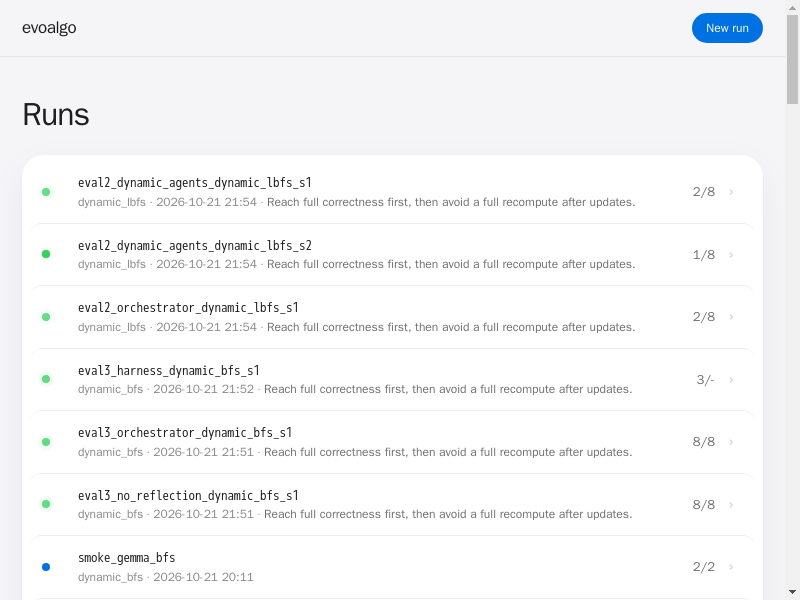
\includegraphics[width=\textwidth]{../campaign/ui_check/01_runs.png}
\caption{The run list. Each row shows the run id, the pack, the last update
time, the research goal, the generation counter, a fitness sparkline, and the
best work ratio. The \textbf{New run} button starts a launch.}
\label{fig:ud-runs}
\end{figure}

\begin{figure}[H]
\centering
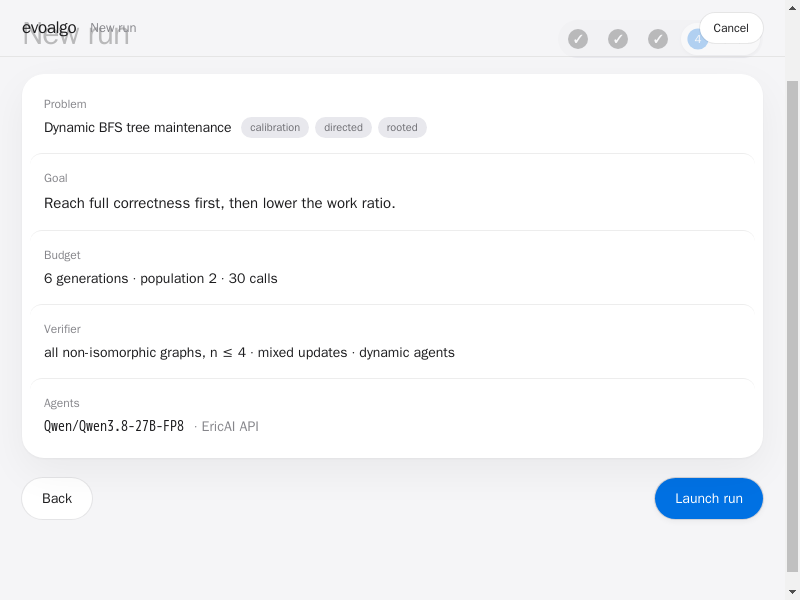
\includegraphics[width=\textwidth]{../campaign/ui_check/03_review.png}
\caption{The Review step of the New Run form for a dynamic BFS run: the chosen
pack and its tags, the goal, the budget (6 generations, population 2, 30
calls), the verifier (all non-isomorphic graphs, $n \le 4$, mixed updates,
dynamic agents), and the agent (Qwen3.8-27B-FP8 over the EricAI API). The
stepper at the top marks the first three steps done.}
\label{fig:ud-review}
\end{figure}

\subsection{Monitor a run live}
\label{sec:ud-monitor}

The live view (Figure~\ref{fig:ud-live}) streams the run's event log over a
websocket and renders, from the top down: a status line (generation, best
candidate, work ratio, and the active hint if any); four KPI tiles (best
fitness, best work ratio, pass rate, model calls) each with a sparkline; a
work-ratio chart (best and mean per generation); a lineage chart (candidates
and their parents); the event log (every agent call, verification, commit, and
cull with its duration); the population table (candidate, parent, role,
fitness, work ratio); the failure-patterns panel (failures grouped by kind and
by the size of the first failing graph); and, when dynamic agents are on, the
specialist-agents panel.

\begin{enumerate}
  \item Open a running run from the list.
  \item Watch the KPI tiles and the event log update as generations commit.
  \item Switch to the failure-patterns panel to see why candidates are failing.
\end{enumerate}

\emph{Expected result:} the view tracks the run in real time; a committing
generation updates the best fitness and work ratio and appends events.
\emph{Recovery:} if the view shows the run as \emph{offline} or
\emph{interrupted}, the engine process is gone; Section~\ref{sec:ud-trouble}
covers resuming. The command-line equivalent is \texttt{evoalgo status
<run\_dir>}.

\begin{figure}[H]
\centering
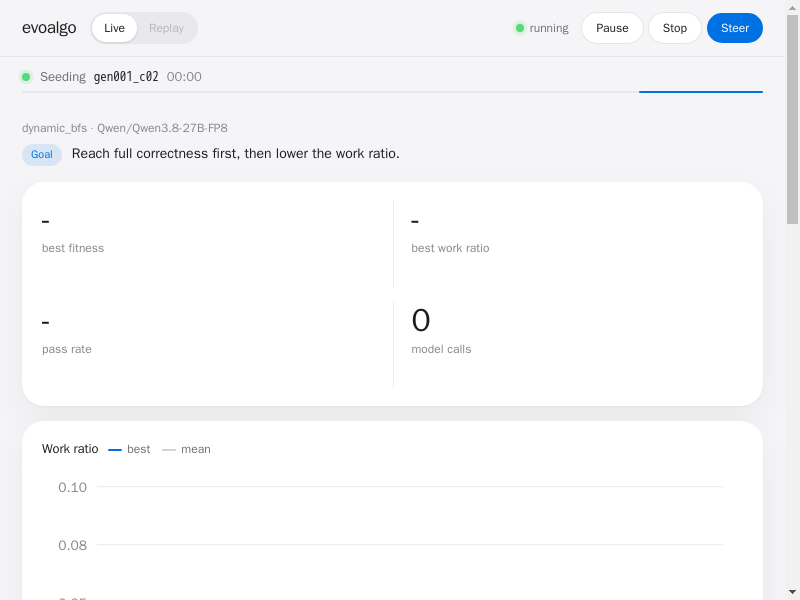
\includegraphics[width=\textwidth]{../campaign/ui_check/04_live.png}
\caption{The live view at the start of a run: the status line reads
\emph{Seeding gen001\_c02}, the four KPI tiles are empty (no committed
generation yet), and the work-ratio chart is waiting for data. The Live/Replay
toggle, the running status, and the Pause, Stop, and Steer controls are at the
top.}
\label{fig:ud-live}
\end{figure}

\subsection{Steer a running run}
\label{sec:ud-steer}

Steering changes the search without restarting it. The controls are the
\textbf{Pause}, \textbf{Stop}, and \textbf{Steer} buttons at the top of the run
page, and the Steer panel (Figure~\ref{fig:ud-done} shows it open over a
finished run).

\begin{enumerate}
  \item Click \textbf{Steer}. The panel offers a \emph{Hint} field (free text,
  up to 2000 characters), a \emph{Call budget} field, and a \emph{Population}
  field.
  \item Enter a hint, a new budget, or a new population, and click
  \textbf{Apply at next generation}. A hint is carried into every subsequent
  agent call; an empty hint clears it.
  \item To pause, click \textbf{Pause}; the engine applies it before the next
  model call and the status moves to \emph{paused}. Click \textbf{Resume} to
  continue. \textbf{Stop} ends the run at the next generation boundary,
  committing whatever was produced.
\end{enumerate}

\emph{Expected result:} each command is acknowledged by the engine with a
\texttt{control\_ack} event, which appears in the event log; the hint is shown
in the status line of the generation it is applied at. \emph{Recovery:} a
command sent to an ended run is refused (\texttt{control\_reject}); the event
log shows the refusal and the run state. The command-line equivalent is
\texttt{evoalgo control <run\_dir> hint "text"}, \texttt{... set
population\_size 4}, \texttt{... pause}, \texttt{... resume}, or \texttt{...
stop}.

\subsection{Replay the generation history}
\label{sec:ud-replay}

\begin{enumerate}
  \item On a finished run, click the \textbf{Replay} toggle.
  \item Drag the generation scrubber to a generation, or press the play button
  to step through generations one by one.
  \item The KPIs, charts, population, and failure patterns re-render for the
  scrubbed generation.
\end{enumerate}

\emph{Expected result:} the view shows the committed state at the chosen
generation, including any hint that was applied there. \emph{Recovery:} replay
is read-only over committed checkpoints; if a generation is missing, the run
was stopped before committing it (see
Section~\ref{sec:ud-trouble}). The command-line equivalent is
\texttt{evoalgo export <run\_dir>}, which writes the per-candidate history to
CSV.

\subsection{Inspect a candidate}
\label{sec:ud-inspect}

\begin{enumerate}
  \item In the population table, the lineage chart, or the failure-patterns
  panel, click a candidate.
  \item The drawer opens (Figure~\ref{fig:ud-faildrawer}) showing the
  candidate's metrics (fitness, work ratio, tests passed over total, parent),
  its failing case when it failed (the operation, the graph size, and the
  expected versus actual value), its reflection when one was written, and its
  full source code.
\end{enumerate}

\emph{Expected result:} the drawer shows the code and, for a failure, the first
failing case that the verifier located. \emph{Recovery:} the drawer loads the
candidate file from the run directory; if the file is absent the candidate was
culled and its code is no longer kept. The command-line equivalent is to open
\texttt{<run\_dir>/candidates/<id>.py}.

\begin{figure}[H]
\centering
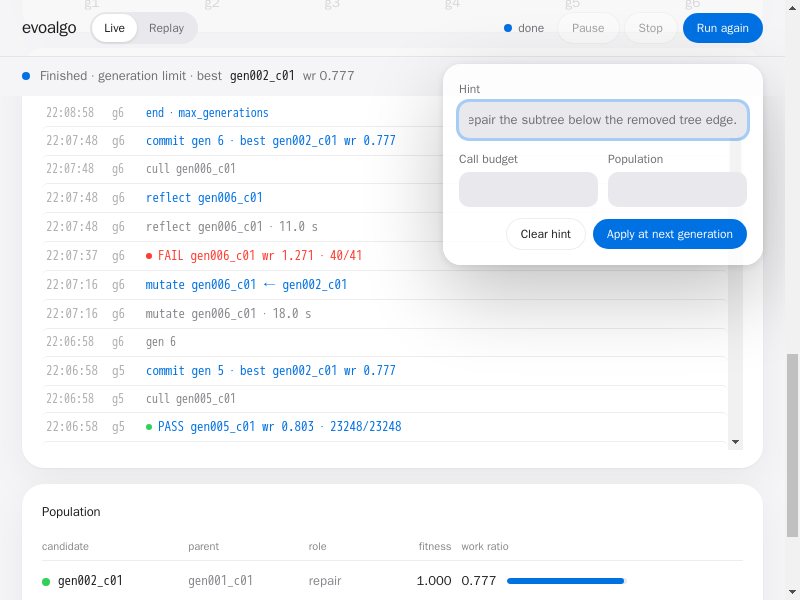
\includegraphics[width=\textwidth]{../campaign/ui_check/06_done.png}
\caption{A finished run with the Steer panel open. The status line reads
\emph{Finished $\cdot$ generation limit $\cdot$ best gen002\_c01 wr 0.777};
the event log shows the generation 6 commits, culls, and a FAIL with its first
failing case; the population table lists the best candidate. The Steer panel
offers a hint, a call budget, and a population, with \emph{Clear hint} and
\emph{Apply at next generation}.}
\label{fig:ud-done}
\end{figure}

\begin{figure}[H]
\centering
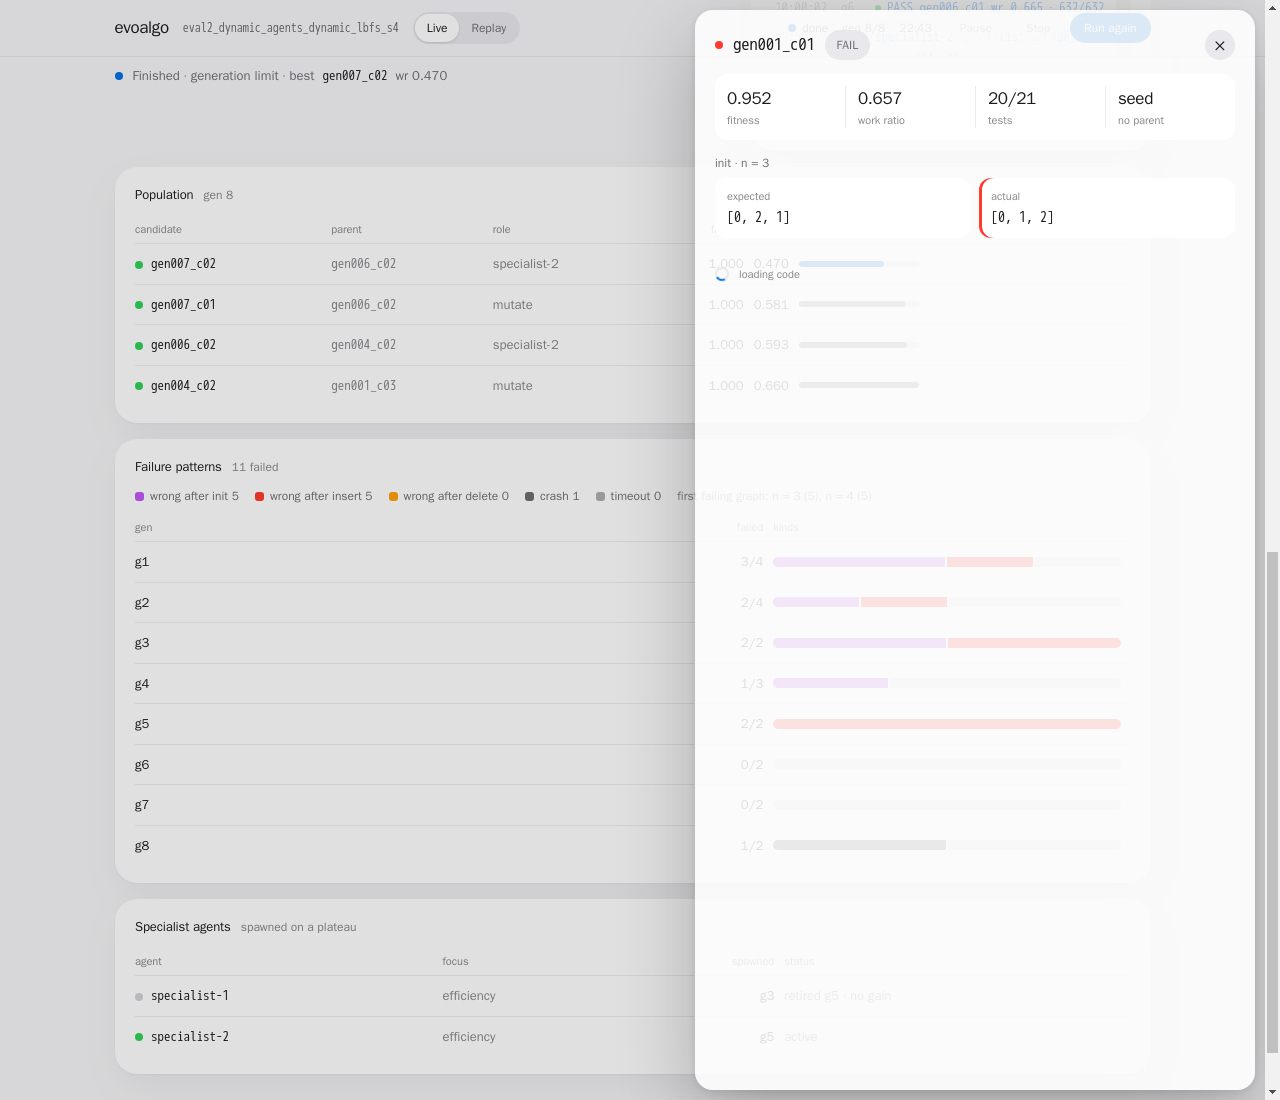
\includegraphics[width=\textwidth]{../campaign/ui_check/09_failure_drawer.png}
\caption{The candidate drawer over a finished dynamic LBFS run. The header shows
the candidate id and its FAIL state; the metrics row shows fitness, work ratio,
tests (20/21), and the role (seed, no parent). The failing case shows the
operation (\texttt{init} at $n = 3$) with the expected and actual values.
Behind the drawer are the population, the failure-patterns panel (11 failed,
grouped by kind and by first-failing size), and the specialist-agents panel
(specialist-1 retired, specialist-2 active).}
\label{fig:ud-faildrawer}
\end{figure}

\subsection{Command-line-only operation}
\label{sec:ud-cli}

The full command set, with the equivalent of every web action:

\begin{enumerate}
  \item \textbf{Configure and start.}
  \texttt{evoalgo configure --problem dynamic\_bfs} with \texttt{-o
  config.yaml}, then \texttt{evoalgo start config.yaml --run-id myrun}.
  \item \textbf{Status.} \texttt{evoalgo status runs/myrun} (add
  \texttt{--json} for a machine-readable summary including the final grade and
  the best candidate path).
  \item \textbf{Control.} \texttt{evoalgo control runs/myrun hint "text"},
  \texttt{... set model\_call\_budget 100}, \texttt{... pause},
  \texttt{... resume}, \texttt{... stop}.
  \item \textbf{Resume.} \texttt{evoalgo resume runs/myrun} reloads the last
  committed generation and continues; a harness workspace is refused here and
  must be continued with \texttt{evoalgo check}.
  \item \textbf{Export.} \texttt{evoalgo export runs/myrun} writes
  \texttt{results/run\_summary.json} and
  \texttt{results/efficiency\_report.csv}.
  \item \textbf{History.} \texttt{evoalgo history} lists previous runs with
  generation, best fitness, best work ratio, pass count, and problem.
\end{enumerate}

\emph{Expected result:} each command prints a short summary; \texttt{start}
prints the final run summary. \emph{Recovery:} a refused or invalid command
prints the reason and exits non-zero without starting a run.

\subsection{The coding-agent harness}
\label{sec:ud-harness}

The harness exposes the same verifier to an external coding agent. The agent
edits one file; the tool grades it and records each grade as a run.

\begin{enumerate}
  \item \textbf{Initialize a workspace.} \texttt{evoalgo init dynamic\_bfs}
  (optionally a target directory, \texttt{--goal}, \texttt{--harness}, and
  \texttt{--max-checks}). This creates \texttt{program.md} (the instructions),
  \texttt{candidate.py} (a starter), and \texttt{results.tsv}, and starts a
  live run shown in the interface.
  \item \textbf{Let the agent work.} The agent edits \texttt{candidate.py} and
  runs \texttt{evoalgo check} (default level \texttt{search}, $n \le 4$), or
  \texttt{check --level examples} ($n \le 3$) for a cheaper check, or
  \texttt{check --level full} ($n \le 5$). The command prints a JSON report and
  exits 0 on PASS, 3 on FAIL, 2 on error.
  \item \textbf{Final grade.} When the agent is satisfied it runs
  \texttt{evoalgo check --final}, the tool's independent re-grade of the kept
  candidate on the full bound. This is the one final grade; repeating it is
  refused.
  \item \textbf{Finish.} \texttt{evoalgo finish} closes the workspace run.
\end{enumerate}

\emph{Expected result:} each check is logged to \texttt{results.tsv} and to the
run folder; the final verdict is the \texttt{--final} re-grade.
\emph{Recovery:} grading a file other than \texttt{candidate.py}, exceeding
\texttt{max\_checks}, or repeating \texttt{--final} is refused with a named
reason. The final grade takes about 10 minutes on BFS/DFS; give the command at
least 15 minutes (Section~\ref{sec:ud-trouble}).

Each \texttt{check} prints a JSON report the agent reads: the verdict
(\texttt{PASS} or \texttt{FAIL}), the grade level, the tests passed over total,
the work ratio, and, on a failure, the first failing case. The tool also stores
a SHA-256 snapshot of the graded \texttt{candidate.py}; if the file is edited
after a grade, the report marks that snapshot as not intact, so a later
\texttt{--final} is a re-grade of the file as it was when it was kept, not of a
file the agent has since changed. The levels are ordered by cost:
\texttt{examples} ($n \le 3$) is a few seconds, \texttt{search} ($n \le 4$) is
the default and also a few seconds, and \texttt{full} ($n \le 5$) is the
minutes-long final grade. An agent typically iterates on \texttt{search} and
finishes with one \texttt{--final}.

The same harness is packaged as an Agent Skill \citep{agentskills}. Inside the
repository it is picked up automatically from \texttt{.agents/skills} and
\texttt{.claude/skills}; elsewhere it is installed with
\texttt{evoalgo skill --install}, which copies it to the home directory's
\texttt{.agents/skills} and \texttt{.claude/skills} (or \texttt{--project}
into the current repository). Once installed, a coding agent can be asked, for
example, to use the evoalgo skill to find a dynamic BFS algorithm for the
\texttt{dynamic\_bfs} pack, and each session appears as a run in
\texttt{evoalgo ui}.

\subsection{The verifier self-test as a user}
\label{sec:ud-verify}

The self-test checks the verifier itself, not a candidate: it runs the
known-good references (which must pass), every seeded fault (which must be
rejected), and the equivalent controls (which must be accepted), over the
bounded universe.

\begin{enumerate}
  \item Run \texttt{evoalgo verify --problem dynamic\_bfs --n-max 3} (a small
  bound for a quick check; the default for the corpus problems is 5).
  \item Read the summary table and the final line.
\end{enumerate}

The command was run at $n \le 3$ and its final lines are:

\begin{lstlisting}[language=bash, basicstyle=\ttfamily\small]
  Zero-false-negative (n<=3): 14/14 real faults rejected -> PASS
  Known-good accepted: PASS
  Equivalent controls accepted: PASS

  Verifier self-test: ALL PASS
\end{lstlisting}

\emph{What ALL PASS means:} every reference and control was accepted and every
seeded fault was rejected at the stated bound, so the verifier is not
permissive (it rejects wrong candidates) and not over-strict (it accepts valid
variants). It is a bounded check, not a proof. The full $n \le 5$ self-test for
BFS, DFS, and LBFS is reported in Chapter~\ref{ch:testing}; the command-line
\texttt{--relabels 2} flag reproduces the full documented universe.

\section{The three complex features, from the user's view}
\label{sec:ud-features}

The three registered contributions are used through the workflows above; this
section states, for each, the user goal, the preconditions, the steps, the
visible result, and the failure recovery, without repeating the step lists.

\subsection{Feature C1: the research tool interface}

\emph{Goal:} launch, monitor, and replay a multi-generation run end to end from
one place. \emph{Preconditions:} an installed package with the \texttt{ui}
extra, a run directory root, and (for an API run) a model key in the named
environment variable. \emph{Steps:} launch from the New Run page
(Section~\ref{sec:ud-launch}), monitor live (Section~\ref{sec:ud-monitor}),
steer (Section~\ref{sec:ud-steer}), and replay (Section~\ref{sec:ud-replay}).
\emph{Visible result:} the live view with KPIs, charts, population, failure
patterns, and specialists; the replay scrubber; and the candidate drawer.
\emph{Failure recovery:} a refused launch names its blocking field; an
interrupted run is resumed (Section~\ref{sec:ud-trouble}); a missing token is
recovered from the printed link or \texttt{runs/.ui-link}.

\subsection{Feature C2: the isomorphism-aware verifier}

\emph{Goal:} trust a candidate's correctness and measure its efficiency.
\emph{Preconditions:} a Linux host with user namespaces (or an explicit
\texttt{EVOALGO\_SANDBOX=none}), and the committed \texttt{nauty} data.
\emph{Steps:} the verifier runs automatically on every candidate during a run
and on the best candidates at the end; the user-facing action is the self-test,
\texttt{evoalgo verify} (Section~\ref{sec:ud-verify}). \emph{Visible result:}
each candidate's state (PASS, FAIL, or CRASH), its fitness, its work ratio, and
its first failing case in the drawer; the self-test's \texttt{ALL PASS} line.
\emph{Failure recovery:} a CRASH or TIMEOUT is a located failure, not a silent
pass; a sandbox that cannot start fails closed with a named error
(Section~\ref{sec:ud-trouble}).

\subsection{Feature C3: cooperative and dynamic agents}

\emph{Goal:} let specialized agents repair candidates, and spawn new
specialists when the search plateaus, without human intervention.
\emph{Preconditions:} a model endpoint (or mock), and, for dynamic agents, the
\emph{spawn a specialist agent when the search plateaus} toggle on the New Run
page (or \texttt{dynamic\_agents: true} in the config). \emph{Steps:} launch
with the toggle; the orchestrator runs the generator, reflector, and repairer
roles, and on a plateau spawns a specialist whose focus is written from the
plateau, retires it after its budget or a window without gain.
\emph{Visible result:} the specialist-agents panel (spawned, focus, status) and
specialist-labelled candidates in the population. \emph{Failure recovery:} a
run with no plateau never spawns a specialist, which is correct; a specialist
that does not improve the search is retired and the run continues.

\section{Results and files}
\label{sec:ud-results}

Every run is a directory under the workdir (default \texttt{runs/}). For a
finished run the directory contains, and the user reads, the following:

\begin{itemize}
  \item \texttt{config.yaml} : the validated configuration actually used.
  \item \texttt{events.jsonl} : the event log, one JSON object per line, with
  contiguous sequence numbers. It is the source for the live view, the replay,
  and the status command.
  \item \texttt{generation\_NNNN.json} : one checkpoint per committed
  generation, holding that generation's candidates, fitness, work ratios, and
  parents. \texttt{COMMITTED} holds the highest committed generation number.
  \item \texttt{candidates/} : the source code of each candidate, one
  \texttt{<id>.py} per candidate.
  \item \texttt{reflections/} : the reflector's failure analysis, one
  \texttt{<id>.md} per reflected candidate.
  \item \texttt{prompt\_logs/} : one JSON file per agent call (role, model,
  duration, token usage, tool calls), for auditing what the model was asked.
  \item \texttt{results/run\_summary.json} and
  \texttt{results/efficiency\_report.csv} : written by \texttt{evoalgo export};
  the summary holds the run id, total generations and candidates, best fitness,
  best candidate id, best work ratio, and pass count; the CSV holds one row per
  candidate with generation, fitness, work ratio, state, timeout flag, and
  tests passed over total.
  \item \texttt{dashboard/} : an HTML snapshot per \texttt{dashboard\_interval}
  generations, for a static view without the live server.
\end{itemize}

The mock run's \texttt{run\_summary.json} was:

\begin{lstlisting}[language=bash, basicstyle=\ttfamily\small]
{
  "run_id": "smoke_mock",
  "total_generations": 1,
  "total_candidates": 2,
  "best_fitness": 1.0,
  "best_candidate_id": "gen001_c01",
  "best_work_ratio": 0.4299706170421156,
  "passing": 2
}
\end{lstlisting}

Reading the numbers: \emph{fitness} is 1.0 for a candidate that passed its
grade and below that otherwise, so the best fitness tells you whether a correct
candidate was found at all. The \emph{work ratio} is the candidate's time over
the offline recomputation baseline on the graded graphs; below 1 means the
candidate is cheaper than recomputing, and it is the number the search optimizes
after correctness. A run uses two grades (Refinement R3 in
Chapter~\ref{ch:requirements}): every candidate is graded during the run on the
small search bound ($n \le 4$ by default), and the best passing candidates are
graded again at the end on the full bound ($n \le 5$). The search grade is fast
and is what the KPIs track live; the final grade is the one that determines the
run's verdict, and a candidate can pass the search grade yet fail the final
grade on a fault that only appears at $n = 5$. The \texttt{final\_graded} event
in \texttt{events.jsonl} records that verdict, and the \texttt{--json} form of
\texttt{status} surfaces it together with the best candidate path.

To export a run, run \texttt{evoalgo export <run\_dir>}; it prints
\texttt{Exported to <run\_dir>/results/} and the two files it wrote. The
\texttt{--json} form of \texttt{status} adds the final grade and the best
candidate path, which is convenient for a supervisor reviewing a run
programmatically.

\section{Troubleshooting, limitations, and FAQ}
\label{sec:ud-trouble}

Table~\ref{tab:ud-trouble} lists the common failures, each verified against the
source or a run. The \emph{Resolution} column gives the safe fix.

\begin{scriptsize}
\setlength{\tabcolsep}{4pt}
\begin{longtable}{@{}p{0.26\textwidth}p{0.34\textwidth}p{0.34\textwidth}@{}}
\caption{Troubleshooting guide (verified cases).}\label{tab:ud-trouble}\\
\toprule
\textbf{Symptom} & \textbf{Cause / diagnosis} & \textbf{Resolution and recovery} \\
\midrule
\endfirsthead
\toprule
\textbf{Symptom} & \textbf{Cause / diagnosis} & \textbf{Resolution and recovery} \\
\midrule
\endhead
\bottomrule
\endfoot
\texttt{the sandbox needs Linux user namespaces (unshare)}; the run refuses to start. & The host has no unprivileged user namespaces, or \texttt{unshare} is missing; the sandbox fails closed. & Enable unprivileged user namespaces on the host. For debugging only, set \texttt{EVOALGO\_SANDBOX=none}, which runs candidates unconfined at the user's own risk. \\
\addlinespace[2pt]
\texttt{API key not found: export ERICAI\_ACCESS\_TOKEN}. & The \texttt{api} backend could not read the key variable. & Export the named variable before starting (\texttt{export ERICAI\_ACCESS\_TOKEN=...}); only the name is stored, the value is read at call time. \\
\addlinespace[2pt]
A run stalls or fails with an auth error on EricAI. & The EricAI token is short-lived and expired. & The token is re-read from \texttt{\textasciitilde/.ericai\_token\_env} on every call and refreshed automatically about 10 minutes before expiry; if the automatic refresh fails, run \texttt{ericai --ericsson-access-token} interactively once. \\
\addlinespace[2pt]
\texttt{missing or wrong access token: open the link printed by evoalgo ui}. & The browser has no valid token cookie. & Open the printed link (or the one in \texttt{runs/.ui-link}); it sets an HttpOnly cookie. The link is single-use per server and dies when the server stops. \\
\addlinespace[2pt]
A run is shown as \emph{interrupted} in the UI. & The engine process exited (crash, host reboot, or a stop). & Run \texttt{evoalgo resume <run\_dir>}; it discards any incomplete generation and continues from the last committed checkpoint. \\
\addlinespace[2pt]
A candidate is \texttt{TIMEOUT}, \texttt{CRASH}, or \texttt{FAIL}. & The candidate hung, raised an exception, or violated the invariant, respectively. & All three are failures, never passes. The drawer shows the located failing case (graph, operation, expected vs actual); use it to steer with a hint. \\
\addlinespace[2pt]
\texttt{evoalgo check --final} appears to hang or is killed by a shell timeout. & The final grade on the full bound takes about 10 minutes for BFS/DFS. & Give the command at least 15 minutes; the workspace brief and the skill now state this. The grade is bounded and will finish. \\
\addlinespace[2pt]
The run stops early with a budget stop reason. & The \texttt{model\_call\_budget} was used. & Raise the budget on the New Run page or via \texttt{evoalgo control <run\_dir> set model\_call\_budget N}, then resume. \\
\addlinespace[2pt]
\texttt{evoalgo ui} fails to bind the port. & Port 8765 is already in use. & Start with \texttt{--port <other>}; the access link is printed for that port. \\
\addlinespace[2pt]
\texttt{check budget used up (N checks); run evoalgo check --final, then evoalgo finish}. & \texttt{max\_checks} was reached. & Run the one final grade, then \texttt{evoalgo finish}; further checks are refused by design. \\
\addlinespace[2pt]
A launch is blocked with \texttt{enlcode not found on this machine}. & The harness agent binary is not on the path. & Install the harness or choose an API endpoint instead; the New Run page names the missing prerequisite. \\
\addlinespace[2pt]
\texttt{evoalgo ui} prints \texttt{The UI needs the 'ui' extra}. & The package was installed without the \texttt{ui} extra. & Reinstall with \texttt{pip install -e '.[ui]'} (or \texttt{'.[api,ui]'}). \\
\bottomrule
\end{longtable}
\end{scriptsize}

\subsection{Limitations}

These are stated plainly so a user does not over-read a result.

\begin{itemize}
  \item \textbf{Bounded verification is not a proof.} A candidate that passes
  has no counterexample within the stated bound ($n \le 5$ by default); a fault
  that only appears on a larger graph is not caught. The word ``proof'' is
  reserved for a mathematical or formal proof, which is out of scope.
  \item \textbf{The bound is small.} The exhaustive universe is $n \le 5$;
  beyond it the verifier uses seeded random sampling, so coverage past the
  bound is sampled, not exhaustive.
  \item \textbf{Model sampling is not seeded.} The test universe and parent
  selection are reproducible, but the language model's sampling is not; two
  runs with the same configuration do not produce identical fitness
  trajectories.
  \item \textbf{Linux only for the jail.} The sandbox requires Linux user
  namespaces; on other platforms it fails closed unless explicitly disabled.
  \item \textbf{Single user, loopback.} The interface binds to 127.0.0.1 and is
  intended for one researcher on one host; there is no multi-user service and
  no enforced read-only role.
\end{itemize}

\subsection{Frequently asked questions}

\begin{description}
  \item[Do I need to install nauty or graph data?] No. The representative
  digraph files are committed in the repository; the tool only reads them.
  \item[Can I run a search without a model key?] Yes. Set
  \texttt{provider: mock}; the mock writes a known-good recompute candidate, so
  a small run finishes in seconds and exercises the whole pipeline. It is for
  trials and demos, not for discovery.
  \item[What does a work ratio below 1 mean?] The candidate is cheaper than
  recomputing the result from scratch on the graded graphs; it is the efficiency
  signal the search optimizes after correctness.
  \item[Is a passing candidate proven correct?] No. It has no counterexample
  within the stated bound ($n \le 5$ by default). That is bounded exhaustive
  verification, not a proof (Refinement R3).
  \item[Can I run two runs at once?] Yes; each run is its own directory and the
  sandbox gives every candidate its own namespace and resource budget. The web
  interface lists both and you switch between them.
  \item[Where do my runs go, and how do I remove them?] Under the workdir
  (default \texttt{runs/}); delete the run directory to remove it, as described
  in Section~\ref{sec:ud-security}.
\end{description}

\section{Security, privacy, backup, and data removal}
\label{sec:ud-security}

\subsection{What is sent to the model provider}

When the \texttt{api} backend is used, each agent call sends the problem brief
(the pack's \texttt{brief.md}), the candidate code being generated or repaired,
the first failing case when repairing, and any active hint. No user files, no
host configuration, and no credentials are sent. The API key is read from the
environment at call time and is never written to a config, a log, or a
prompt; the configuration stores only the variable \emph{name}
(\texttt{api\_key\_env}). Auth errors are logged with the status and the
provider's error code only, not the response body, so a key echoed by a
provider is not captured in the (committed) call log.

\subsection{Sandbox guarantees, in user terms}

Candidate code is model-written and untrusted. It runs inside a Linux
namespace jail: no network (the network namespace is down), no home directory
or token files (the home, shared, and temp trees are hidden behind an empty
tmpfs and the interpreter's import paths are bound back read-only), its own pid
namespace, and its own IPC namespace so shared memory does not outlive the
candidate. Resource limits are enforced before any candidate code runs: 4 GB of
address space, CPU time equal to the wall-clock timeout plus 5 seconds, 4
processes, 16 MB per file, 64 open files, 256 MB of result output, and 64 KB of
stderr. A candidate that tries to read a secret, reach the network, or exhaust
the host is blocked and reported as a failure, not a pass. Where the jail is
unavailable the sandbox refuses to run unless \texttt{EVOALGO\_SANDBOX=none} is
set, which removes these guarantees and is for debugging only.

\subsection{Secrets handling}

The only secret the tool touches is the model API key, and it is handled by
name: the config and the New Run page store and show the variable name and
whether a value is present, never the value. The EricAI token file
(\texttt{\textasciitilde/.ericai\_token\_env}) is created with mode 600 and
refreshed under a file lock so parallel runs refresh once between them. The UI
access token is generated per server, printed once (or written to
\texttt{runs/.ui-link} with mode 600 when output is redirected), and deleted
when the server stops.

\subsection{Backup and data removal}

There is no database and no remote store: a run is fully described by its
directory under the workdir. To back up a run, copy its directory; to remove
it, delete the directory. Deleting a run directory removes its candidates,
reflections, prompt logs, checkpoints, event log, and exported results
together, and the run disappears from the interface list and from
\texttt{evoalgo history}. The \texttt{runs/.ui-link} file is removed
automatically when the server stops. Nothing is written outside the workdir
except the EricAI token file in the home directory and the installed Agent
Skill in \texttt{\textasciitilde/.agents/skills} or
\texttt{\textasciitilde/.claude/skills} (removed by deleting those directories).


\part{Developer Documentation}
\chapter{Requirements Specification}
\label{ch:requirements}

This chapter is the single canonical requirements baseline for the thesis. It
states every requirement against the system as it is implemented at the current
source revision. Requirement identifiers (\texttt{FR-*}, \texttt{NFR-*}) are
stable and are the keys used by the traceability matrix in
Section~\ref{sec:traceability} and by the test-evidence families in the testing
chapter.

\section{System context, stakeholders, assumptions, and constraints}
\label{sec:context}

\subsection{System context}

The system is a research tool for discovering correct and efficient
\emph{dynamic} graph algorithms. A dynamic algorithm maintains a structural
result (a BFS tree, a DFS tree, a lexicographic BFS ordering, a strongly
connected component partition, or a reachability set) incrementally under edge
insertions and deletions, instead of recomputing it from scratch after every
change. The tool combines LLM-based code generation and repair with exhaustive,
isomorphism-aware verification inside an evolutionary search loop, and reports
both positive and negative results.

The system has one trusted side and many untrusted ones. The verifier, the
sandbox, and the evolutionary orchestrator are pre-built and trusted. Candidate
algorithms are untrusted Python written by an LLM; they execute only inside the
sandbox jail and are never given access to the verifier, the test graphs, the
oracle, or the host. That boundary is the central design constraint, stated as
a requirement in Section~\ref{sec:fr-ver} and \ref{sec:fr-sbx}.

The system is a Python package (\texttt{evoalgo}) with a command-line
interface, a local web user interface served from the same package, and a
harness mode in which an external coding agent drives the search while the
system only grades and records. There is no database; all state is JSON,
line-delimited JSON, and CSV under a per-run directory.

\subsection{Stakeholders}

\begin{itemize}
  \item \textbf{Researcher.} Configures and launches runs, monitors and steers
  them, inspects candidates, replays generation history, exports results, and
  runs the verifier self-test. The researcher is the primary actor and the one
  who interprets outcomes.
  \item \textbf{Supervisor.} Reviews run status, exported artefacts, and the
  verification evidence; audits the verifier and its acceptance evidence.
  \item \textbf{External coding agent.} In harness mode, a coding agent
  (for example enlcode, Claude Code, or Codex) edits the single candidate file
  and calls \texttt{evoalgo check}; the system grades and records each check.
  \item \textbf{LLM provider} (secondary actor). A hosted or local
  OpenAI-compatible model API, or an agent harness backend, that supplies the
  model calls for the generation, repair, and reflection roles.
\end{itemize}

\subsection{Assumptions}

\begin{itemize}
  \item A reachable model provider (hosted or local) is available for the
  duration of a run, or a scripted mock backend is used for offline tests.
  \item The host operating system is Linux with unprivileged user namespaces
  enabled, so the sandbox jail can be built. On a host without them the sandbox
  refuses to run unless explicitly disabled (see \texttt{FR-SBX-05}).
  \item The \texttt{nauty} graph data files are committed in the repository
  (\path{src/evoalgo/data/nauty/}); the \texttt{nauty} command line is not
  required at run time, only the pre-generated representative files.
  \item Dynamic outputs (BFS/DFS trees, orderings, partitions) are not unique;
  correctness is judged by an invariant or certificate, not by equality to a
  single reference output (Refinement R1, Section~\ref{sec:refinements}).
\end{itemize}

\subsection{Constraints}

\begin{itemize}
  \item \textbf{Platform.} Linux only, for the sandbox jail (namespaces and
  \texttt{mount\_setattr}). Python 3.11 or later.
  \item \textbf{No database.} Persistence is files only (JSON, JSONL, CSV).
  \item \textbf{No network for candidates.} Candidate code runs with the
  network namespace down; the verifier and agents use the network, the
  candidate never does.
  \item \textbf{Bounded verification.} Correctness is established by exhaustive
  finite testing within a stated graph-size and sequence bound, not by a
  proof (Refinement R3). The word ``proof'' is reserved for a mathematical or
  formal proof, which is out of scope.
\end{itemize}

\subsection{Non-goals}

\begin{itemize}
  \item A formal proof of correctness of a discovered algorithm beyond the
  stated bound. The Lean~4 formalisation step exists in the code but is
  experimental and never gates a run; it is not a committed deliverable.
  \item A general program synthesizer. The system targets a fixed set of
  dynamic graph problems with a fixed candidate interface; it does not
  synthesize arbitrary programs.
  \item A multi-user or remote service. The web UI binds to the loopback
  address and is intended for a single researcher on one host.
  \item Guaranteeing an efficiency improvement. The search may return a
  correct algorithm that is not faster than recomputing; that is a valid,
  reported outcome, not a failure.
\end{itemize}

\section{Use-case model}
\label{sec:usecases}

Figure~\ref{fig:use-cases} gives the use-case view.\footnote{The TikZ source of this figure was written with AI assistance (Claude Opus 5.5, Qwen3.8-27B) and checked against the code; see Section~\ref{sec:ai-use}.} Actors sit outside the
system boundary. White ellipses are triggered by a user or by the external
coding agent; grey ellipses are performed automatically by the system inside
the evolutionary loop or by the harness. \texttt{$\ll$include$\gg$} arrows run
from a base use case to the use case it always includes;
\texttt{$\ll$extend$\gg$} arrows run from an optional extension to the base it
conditions on.

\begin{figure}[H]
\centering
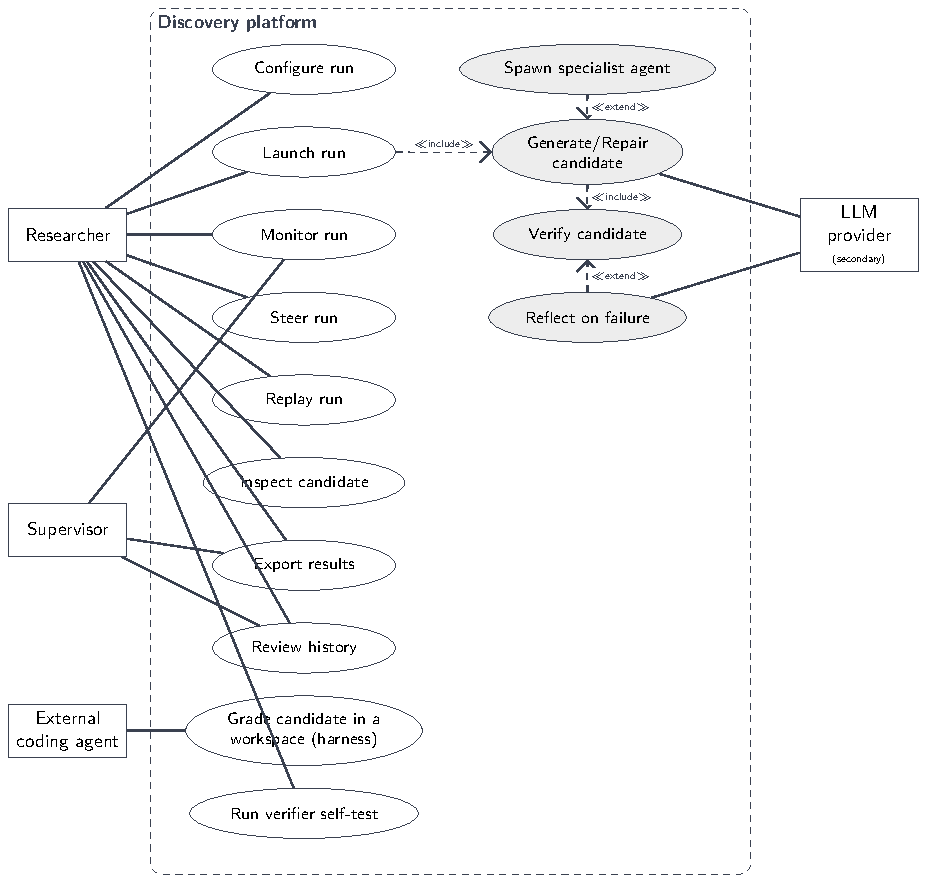
\includegraphics[width=0.85\textwidth]{figures/use-cases.pdf}
\caption{Use case diagram of the discovery platform. White ellipses are
user- or agent-triggered; grey ellipses are automatic. Reflection extends
verification (it runs only on a failure), and specialist spawning extends
generation (it runs only on a plateau).}
\label{fig:use-cases}
\end{figure}

The use cases are \emph{Configure run}, \emph{Launch run}, \emph{Monitor run},
\emph{Steer run}, \emph{Replay run}, \emph{Inspect candidate}, \emph{Export
results}, \emph{Review history}, \emph{Run verifier self-test}, and \emph{Grade
candidate in a workspace (harness)}, plus the internal \emph{Generate/Repair
candidate}, \emph{Verify candidate}, \emph{Reflect on failure}, and \emph{Spawn
specialist agent}. The five most important ones are summarised, each with its
actor, main flow and alternate and failure flows, in Table~\ref{tab:usecases}
(Appendix~\ref{app:tables}); their full narratives are in
Appendix~\ref{app:requirements}.


\section{Functional requirements}
\label{sec:fr}

The functional requirements are atomic and testable, and each has a stable
identifier whose prefix names the capability. There are 60: nine for the command
line and run control (\texttt{FR-CLI-01} to \texttt{09}), nine for the web
interface (\texttt{FR-UI}), eleven for the verification engine
(\texttt{FR-VER}), five for the sandbox (\texttt{FR-SBX}), seven for the agents
(\texttt{FR-AGENT}), ten for the evolutionary loop (\texttt{FR-EVO}), four for
persistence (\texttt{FR-PER}) and five for the harness (\texttt{FR-HAR}).
Table~\ref{tab:fr-summary} (Appendix~\ref{app:tables}) lists them by title and
priority; the full catalogue in Appendix~\ref{app:requirements} gives,
for every requirement, its input, precondition, behaviour, output, error or
rejection behaviour, priority, and acceptance evidence (named tests or campaign
artefacts). Priorities follow MoSCoW: \emph{Must} requirements are the
registered commitments, \emph{Should} and \emph{Could} requirements support them.



\section{Bounded verification universe}
\label{sec:universe}

The coverage claim of the verification engine is a finite, reproducible test
universe, not a proof. This section defines it so a reviewer can calculate its
size and distinguish exhaustive from sampled evidence.

\subsection{Base graphs}

Graphs are simple and loop-free, as an adjacency matrix of zeros and ones. The
base-graph set depends on the problem's direction and rooting:

\begin{itemize}
  \item \textbf{Directed, unrooted problems} use the non-isomorphic digraph
  representatives from the committed \texttt{nauty} data files
  (\texttt{directed\_n$<$n$>$.d6}), one per isomorphism class. The class counts
  for $n = 1$ to $5$ are 1, 3, 16, 218, and 9,608 (OEIS A000273, \citealp{oeisA000273}).
  \item \textbf{Directed, rooted problems} (BFS, DFS, reachability, which fix a
  source at vertex 0) use the rooted representatives
  (\texttt{rooted\_n$<$n$>$.d6}), one per (digraph, root-orbit) class with the
  root relabelled to vertex 0. The class counts for $n = 1$ to $5$ are 1, 4, 36,
  752, and 45,960 (OEIS A353996, \citealp{oeisA353996}).
  \item \textbf{Undirected problems} (MCS, LBFS) use \emph{every} labelled graph
  up to the bound, so the result does not depend on vertex labels. The labelled
  counts for $n = 2$ to $5$ are 2, 8, 64, and 1,024.
\end{itemize}

For directed problems the engine also applies a fixed number of deterministic
random relabellings of each representative (two per class for the final grade, one
for the search grade) to exercise label-dependent behaviour such as id
tie-breaks. A relabelling is isomorphic to its representative, so this adds
coverage of label handling without adding new isomorphism classes.

\subsection{Operation sequences}

For every base graph of size at most the exhaustive-flip bound (5), the universe
contains two kinds of sequences:

\begin{itemize}
  \item \textbf{All legal single-edge flips.} For each possible edge, one
  length-1 sequence that inserts it if absent or deletes it if present. This is
  ``every possible edge operation'' on the base graph: $n(n-1)$ flips for a
  directed graph and $n(n-1)/2$ for an undirected one.
  \item \textbf{Seeded random sequences.} \texttt{seq\_count} sequences of up to
  \texttt{seq\_len\_max} operations, each operation legal on the evolving graph,
  seeded by the bound seed plus the graph size, so the set is reproducible.
\end{itemize}

The defaults are \texttt{bound.n\_max} 5, \texttt{n\_random} 20,
\texttt{seq\_len\_max} 20, \texttt{seq\_count} 10, and \texttt{seed} 1337. The
\texttt{update\_mode} (\texttt{mixed}, \texttt{insert\_only},
\texttt{delete\_only}) filters the sequences to the allowed operation type while
keeping them legal.

\subsection{Exhaustive versus sampled}

Within the stated bound the universe is \emph{exhaustive up to isomorphism} for
directed problems (every non-isomorphic class, plus relabellings) and
\emph{exhaustive over labels} for undirected problems (every labelled graph).
Random sampling (\texttt{n\_random}) is used only for a graph size that has no
committed data file (that is, beyond the bound), so it never reduces coverage
inside the documented bound.

\subsection{Two grades and their exact sizes}

The engine uses two grades. The \emph{search grade} runs during the evolution on
every candidate: non-isomorphic graphs up to \texttt{search\_n\_max} (4), every
single flip, and \texttt{search\_seq\_count} (3) short sequences, with one
relabel per class; it takes seconds per candidate. The \emph{final grade} runs on
the best passing candidates on the full bound: $n \le 5$, every single flip, and
\texttt{seq\_count} (10) sequences of up to \texttt{seq\_len\_max} (20), with two
relabels per class.

The exact final-grade sizes, computed from the committed data files and the
sequence rules above, are:

\begin{center}
\footnotesize
\setlength{\tabcolsep}{6pt}
\begin{tabular}{@{}lrrrrr@{}}
\toprule
Problem & $n{=}2$ & $n{=}3$ & $n{=}4$ & $n{=}5$ & Total sequences \\
\midrule
Dynamic BFS / DFS (directed, rooted) & 96 & 1{,}728 & 49{,}632 & 4{,}136{,}400 & 4{,}187{,}856 \\
Dynamic LBFS (undirected, all labelled) & 22 & 104 & 1{,}024 & 20{,}480 & 21{,}630 \\
\bottomrule
\end{tabular}
\end{center}

These are the figures reported in the evaluation. A candidate that passes the
final grade has no counterexample within this bound; that is bounded exhaustive
verification, and it is not called a proof. The bound is on base graphs and on
the operation histories listed above: all single-edge flips and a finite set of
seeded sequences. It does not cover every internal state a candidate can reach
or arbitrarily long histories, even for $n \le 5$.

\section{Non-functional requirements}
\label{sec:nfr}

Each quality attribute has a measurable target or an explicit statement of what
is and is not asserted. The numbers are taken from the committed code, the test
suite, and the campaign artefacts; none is estimated.

\begin{itemize}
  \item \textbf{Performance.} A final grade of one BFS or DFS candidate on the
  full bound takes about 10 minutes (\texttt{NFR-PERF-01}), and a 1,000-graph
  chunk at $n = 5$ stays near 620 MB resident, inside the 4 GB address-space limit
  (\texttt{NFR-PERF-02}).
  \item \textbf{Security.} Candidate code is isolated from the host, the
  network and the secrets (\texttt{NFR-SEC-01}); secrets are handled by
  variable name only (\texttt{NFR-SEC-02}); the UI is loopback-only and
  token-protected (\texttt{NFR-SEC-03}).
  \item \textbf{Reliability.} A run resumes without losing completed work
  (\texttt{NFR-REL-01}), and transient model-call failures do not abort it
  (\texttt{NFR-REL-02}).
  \item \textbf{Reproducibility, usability, portability, maintainability.}
  The universe and parent selection are reproducible, model sampling is not
  (\texttt{NFR-REPR-01}); the UI is keyboard-usable without a WCAG claim
  (\texttt{NFR-USAB-01}); Linux and Python 3.11 or later
  (\texttt{NFR-PORT-01}); 193 pytest and 14 Vitest tests are the regression
  gate (\texttt{NFR-MAINT-01}).
\end{itemize}

Table~\ref{tab:nfr} in Appendix~\ref{app:tables} gives the measurement, the
threshold and the evidence for each of the eleven.

\section{Acceptance criteria per contribution}
\label{sec:acceptance}

Each registered contribution has a named demonstration or test, an explicit
pass/fail threshold, and a stored evidence artefact. Finite exhaustive testing
establishes bounded correctness within the stated bound; it is not a proof for
arbitrary graph size.

\begin{center}
\footnotesize
\setlength{\tabcolsep}{5pt}
\begin{longtable}{@{}>{\raggedright\arraybackslash}p{0.20\textwidth}>{\raggedright\arraybackslash}p{0.42\textwidth}>{\raggedright\arraybackslash}p{0.34\textwidth}@{}}
\toprule
\textbf{Contribution} & \textbf{Named demonstration / test} & \textbf{Threshold and evidence} \\
\midrule
\endfirsthead
\toprule
\textbf{Contribution} & \textbf{Named demonstration / test} & \textbf{Threshold and evidence} \\
\midrule
\endhead
\bottomrule
\endfoot

C1: research tool UI framework & A run is launched from the web New Run page,
monitored live, steered with a hint (acknowledged by the engine), and its
generation history is replayed with the scrubber, end to end. & The recorded
browser run completes with a final verdict and no error; the hint is acknowledged
at a generation boundary. Evidence: \texttt{ui\_check/01\_runs.png} through
\texttt{ui\_check/09\_failure\_drawer.png} and the recorded run
\texttt{runs/ui\_browser\_e2e\_bfs}. \\
\addlinespace[2pt]

C2: isomorphism-aware verification engine & The verifier self-test on the full
bound for a corpus problem: known-good references and equivalent controls
accepted, every seeded fault and one-line mutation rejected. & Zero false
negatives at $n \le 5$ (every seeded fault of the corpus rejected) and every reference and control
accepted. Evidence: \texttt{selftest\_dfs\_n5.log} (22 faults rejected, including
15 seeded and 7 one-line mutations of the known dynamic DFS reference) and
\texttt{selftest\_lbfs\_n5.log} (12 faults rejected); \texttt{test\_real\_faults\_rejected\_n5},
\texttt{test\_known\_good\_references\_pass\_n5}. \\
\addlinespace[2pt]

C3: cooperative agents with dynamic generation & An unattended orchestrator run
on dynamic BFS reaches a correct candidate, and the dynamic-agent variant spawns
and retires specialists on a plateau. & A search-grade pass is reached within the
configured generations with no human intervention; the final grade of the kept
candidate passes the full bound. Evidence: the campaign runs
(\texttt{eval1} orchestrator arm, 9/9 final-grade PASS) and
\texttt{test\_mock\_run\_spawns\_and\_retires\_a\_specialist},
\texttt{test\_plateau\_on\_fitness\_or\_work\_ratio}. \\
\bottomrule
\caption{Acceptance criteria per registered contribution.}
\label{tab:acceptance}
\end{longtable}
\end{center}

\section{Traceability to the approved proposal}
\label{sec:traceability}

Table~\ref{tab:traceability} traces each registered contribution and deliverable
to the requirement identifiers in this chapter, to the design sections that will
carry them (Chapter~\ref{ch:design}), to the implementation sections
(Chapter~\ref{ch:implementation}), and to the test-evidence families
(Chapter~\ref{ch:testing}). No registered contribution is removed; the four
refinements in Section~\ref{sec:refinements} narrow or re-prioritise the
registered wording and are stated explicitly.

\begin{center}
\footnotesize
\setlength{\tabcolsep}{4pt}
\begin{longtable}{@{}>{\raggedright\arraybackslash}p{0.17\textwidth}>{\raggedright\arraybackslash}p{0.20\textwidth}>{\raggedright\arraybackslash}p{0.25\textwidth}>{\raggedright\arraybackslash}p{0.16\textwidth}>{\raggedright\arraybackslash}p{0.14\textwidth}@{}}
\toprule
\textbf{Commitment} & \textbf{Req.\ IDs} & \textbf{Design} & \textbf{Implem.} & \textbf{Tests} \\
\midrule
\endfirsthead
\toprule
\textbf{Commitment} & \textbf{Req.\ IDs} & \textbf{Design} & \textbf{Implem.} & \textbf{Tests} \\
\midrule
\endhead
\bottomrule
\endfoot

C1: research tool UI framework & \texttt{FR-CLI-01} to \texttt{FR-CLI-09},
\texttt{FR-UI-01} to \texttt{FR-UI-09}, \texttt{FR-PER-01} to \texttt{FR-PER-04} &
\S\ref{sec:design-architecture}, \S\ref{sec:design-ui},
\S\ref{sec:design-concurrency}, \S\ref{sec:design-persistence} &
\S\ref{sec:impl-ui} & TC-UI, TC-SRV, TC-EVO \\
\addlinespace[2pt]

C2: isomorphism-aware verification engine & \texttt{FR-VER-01} to
\texttt{FR-VER-11}, \texttt{FR-SBX-01} to \texttt{FR-SBX-05} &
\S\ref{sec:design-verifier}, \S\ref{sec:design-sandbox},
\S\ref{sec:design-domain} & \S\ref{sec:impl-verifier},
\S\ref{sec:impl-sandbox} & TC-VER, TC-SBX, TC-PER \\
\addlinespace[2pt]

C3: cooperative agents with dynamic generation & \texttt{FR-AGENT-01} to
\texttt{FR-AGENT-06}, \texttt{FR-EVO-01} to \texttt{FR-EVO-10} &
\S\ref{sec:design-agents}, \S\ref{sec:design-architecture},
\S\ref{sec:design-concurrency} & \S\ref{sec:impl-agents} &
TC-AG, TC-EVO \\
\addlinespace[2pt]

Deliverable: tiered evaluation (calibration BFS/DFS to open LBFS) &
\texttt{FR-VER-10}, \texttt{FR-VER-11}, \texttt{NFR-PERF-01} &
\S\ref{sec:design-verifier}, \S\ref{sec:design-domain} &
\S\ref{sec:impl-verifier} & TC-VER; campaign \texttt{analysis.md} \\
\addlinespace[2pt]

Deliverable: harness mode (Refinement R4) & \texttt{FR-HAR-01} to
\texttt{FR-HAR-05}, \texttt{FR-VER-09} & \S\ref{sec:design-agents},
\S\ref{sec:design-sandbox} & \S\ref{sec:impl-agents}, \S\ref{sec:impl-sandbox}
& TC-HAR, TC-SBX \\
\bottomrule
\caption{End-to-end traceability from the registered commitments to
requirements, design, implementation, and test evidence.}
\label{tab:traceability}
\end{longtable}
\end{center}

\section{Refinements of the registered topic}
\label{sec:refinements}

Four refinements relative to the registered wording are stated here so they are
visible and judgeable rather than hidden. None removes a registered contribution.

\begin{description}
  \item[R1: comparison by invariant or certificate, not raw equality.] The
  registered wording compares a candidate's output against offline
  recomputation. Dynamic BFS and DFS outputs are not unique (ties in the
  traversal), so raw equality would reject correct candidates. The offline
  oracle still defines the semantics and is the efficiency baseline (the work
  ratio), but the checker accepts any valid structure: for BFS the parent tree
  and distances are certified, for DFS the parent and discover/finish times are
  certified by laminarity and the absence of a forward-cross edge, and for LBFS
  the ordering is certified by the four-point property. This is a sound
  refinement of the verifier contract, not a change of what is being measured.
  \item[R2: LBFS is undirected.] Lexicographic BFS is defined on undirected
  graphs, so dynamic LBFS runs on undirected graphs (every labelled graph up to
  the bound); BFS, DFS, SCC, and reachability run on directed graphs. The
  registered wording listed LBFS as directed; that is corrected here.
  \item[R3: two-tier grading and bounded verification.] Every candidate is
  graded during the run on the small search bound ($n \le 4$), and the best
  passing candidates are graded on the full final bound ($n \le 5$, 4,187,856
  test sequences for BFS/DFS). A result is reported as bounded exhaustive
  verification, that is no counterexample within the stated bound, and is never
  called a proof.
  \item[R4: the verifier is also exposed as a harness.] Besides the built-in
  orchestrator, the same verifier is exposed to an external coding agent through
  a harness (\texttt{evoalgo init} and \texttt{evoalgo check}, packaged as an
  agent skill). This is an extra mode, evaluated as a baseline against the
  orchestrator, not a replacement for it.
\end{description}

\chapter{Solution Design}
\label{ch:design}

\TemplateGuidance{Aim for at least about 10 substantive pages and 3--4 genuinely
useful figures: for example system context/container architecture, data model or
class diagram, an important interaction sequence, and a UI/navigation or API view.
Every figure needs a legible caption, must be cited and interpreted in the prose,
and should reveal a decision rather than decorate the chapter. Prefer vector PDF;
keep text readable at 100\% and do not use screenshots of diagrams or source code.}

\section{Architectural drivers and overview}
<Connect the architecture to requirement IDs and the three contributions.>

\begin{figure}[H]
  \centering
  \fbox{\parbox[c][45mm][c]{0.82\textwidth}{\centering
    Replace with a legible architecture figure exported as vector PDF.\\
    Explain system boundaries, components, protocols, and trust boundaries.}}
  \caption{System architecture and principal responsibilities (placeholder).}
  \label{fig:architecture}
\end{figure}

Figure~\ref{fig:architecture} must be discussed here: identify the consequential
boundaries and explain why this decomposition satisfies the architectural drivers.

\section{Business rules and domain model}
<Define invariants, state transitions, permissions, and edge cases. Include a class
or domain diagram when required by the consultation checkpoint or project type.>

\section{Data and persistence design}
<Describe schemas, ownership, lifecycle, migrations, consistency, indexing, privacy,
backup, retention, and deletion. Link decisions to requirements and tests.>

\section{Interfaces, API, and interaction design}
<Document contracts, validation, errors, authentication/authorization, versioning,
and one difficult interaction sequence.>

\section{User-interface and accessibility design}
<Explain information architecture, core screens, states, responsive behaviour,
feedback, keyboard use, contrast, and accessibility decisions where applicable.>

\section{Security, privacy, and failure design}
<State assets, trust boundaries, threats, mitigations, degraded modes, and recovery.>

\section{Decisions, alternatives, and trade-offs}
\begin{longtable}{@{}p{0.16\textwidth}p{0.25\textwidth}p{0.24\textwidth}p{0.24\textwidth}@{}}
\caption{Architectural decision summary.}\label{tab:decisions}\\
\toprule
\textbf{Decision} & \textbf{Chosen option and rationale} & \textbf{Rejected alternative} & \textbf{Consequences / evidence} \\
\midrule
\endfirsthead
\toprule
\textbf{Decision} & \textbf{Chosen option and rationale} & \textbf{Rejected alternative} & \textbf{Consequences / evidence} \\
\midrule
\endhead
ADR-01 & <choice and requirement driver> & <credible alternative> & <costs, risks, validation> \\
\bottomrule
\end{longtable}

\chapter{Implementation}
\label{ch:implementation}

\TemplateGuidance{Aim for at least about 10 substantive pages. Explain difficult
implementation work through the three contributions and trace it back to design.
The repository is evidence: submit readable source, reproducible dependency manifests,
meaningful history where available, configuration examples without secrets, static
analysis, and build instructions. A common planning heuristic for UI-centred work is
roughly 2,000--3,000 meaningful student-written lines excluding generated code,
dependencies, and boilerplate; difficulty and substance matter more than raw counts.}

\section{Toolchain, dependencies, and repository structure}
<Identify exact versions, why important libraries were chosen, module ownership,
build/run commands, dependency locking, and repository workflow. Cite tools actually used.>

\section{Implementation of contribution C1}
<Explain the hard part, relevant design, key algorithm or code excerpt, error handling,
and evidence. Keep excerpts short and discuss them; do not paste whole files.>

\section{Implementation of contribution C2}
<Explain the hard part, design link, code-level decisions, and evidence.>

\section{Implementation of contribution C3}
<Explain the hard part, design link, code-level decisions, and evidence.>

\section{Integration, configuration, and operational concerns}
<Cover external services, environment variables, deployment, migrations, logging,
observability, concurrency, resource handling, and recovery where applicable.>

\section{Design deviations and technical debt}
<Name what changed from the approved design, why, its consequences, and any remaining
bugs, shortcomings, or future work. Honest bounded limitations are stronger than vague claims.>

\chapter{Testing and Evaluation}
\label{ch:testing}

\TemplateGuidance{Aim for at least about 10 substantive pages. Test the promises,
not just the happy path. For each case give requirement links, preconditions, data,
steps, expected result, observed result, environment, and evidence. Balance the mix
to the project: user-facing/UI checks, unit or functional tests, integration/E2E tests,
and advanced reliability, security, performance, scalability, usability, or model
evaluation. For AI/data projects, define datasets, baselines, metrics, uncertainty,
and error analysis; do not rely on selected anecdotes.}

\section{Strategy, environment, and evidence policy}
<Define levels, tools, fixtures, versions, coverage boundaries, reproducibility,
and how screenshots/logs/reports are stored. Distinguish automated from manual tests.>

\section{Requirement-based test cases}
\begin{longtable}{@{}p{0.09\textwidth}p{0.14\textwidth}p{0.22\textwidth}p{0.20\textwidth}p{0.20\textwidth}@{}}
\caption{Test-case evidence.}\label{tab:test-cases}\\
\toprule
\textbf{ID} & \textbf{Req.} & \textbf{Setup and steps} & \textbf{Expected} & \textbf{Observed / evidence} \\
\midrule
\endfirsthead
\toprule
\textbf{ID} & \textbf{Req.} & \textbf{Setup and steps} & \textbf{Expected} & \textbf{Observed / evidence} \\
\midrule
\endhead
TC-01 & FR-01 & <environment, data, actions> & <specific result> & <pass/fail, value, artifact> \\
\bottomrule
\end{longtable}

\section{Unit and functional testing}
<Explain representative normal, boundary, error, and property/invariant tests.>

\section{Integration and end-to-end testing}
<Verify real boundaries, persistence, APIs, devices, accounts, or services; document
what had to remain manual and why.>

\section{Non-functional evaluation}
<Report workloads, baselines, measurement method, raw/summary data, thresholds,
variation, and limitations. Avoid performance adjectives without numbers.>

\section{Defects, negative results, and lessons learned}
<Describe significant defects discovered, how they were diagnosed and resolved,
remaining failures, threats to validity, and what the evidence does not establish.>

\chapter{Conclusion}
\label{ch:conclusion}

\TemplateGuidance{Aim for roughly 2--4 substantive pages. Answer the problem stated
in Chapter~\ref{ch:introduction}; assess every approved commitment and success
criterion; synthesize the evidence for C1--C3; state lessons, limitations, and realistic
future work. Do not introduce a new implementation or repeat the abstract.}

\section{Results against commitments and success criteria}
<State fulfilled, partially fulfilled, and unfulfilled commitments with evidence.>

\section{Contribution summary}
<Explain what the three contributions achieved and what the tests/evaluation support.>

\section{Limitations, lessons learned, and future work}
<Prioritize concrete limitations and future steps. Separate necessary remediation
from optional extensions.>


\ifshowtemplateguidance
  % Keep the template's source examples visible until the student starts replacing
  % them. Remove unused entries before final submission.
  \nocite{*}
\fi
\cleardoublepage
\phantomsection
\addcontentsline{toc}{chapter}{Bibliography}
\bibliographystyle{plainnat}
\bibliography{references}

\cleardoublepage
\phantomsection
\addcontentsline{toc}{chapter}{List of Figures}
\listoffigures

\cleardoublepage
\phantomsection
\addcontentsline{toc}{chapter}{List of Tables}
\listoftables

\appendix
\chapter{Build, Run, and Reproducibility Record}
\label{app:reproducibility}

This appendix records how to obtain, build, run, and reproduce the system and
the evidence reported in the thesis; the full user-facing instructions are in
Chapter~\ref{ch:user-documentation}.

\section{Repository, revision, environment, and install}

The source is in a private GitHub repository to which the supervisor has
access, and the complete source is part of the submission archive:

\url{https://github.com/thonmay/ai-dynamic-graph-algorithms}

The thesis describes the code at commit \texttt{7895107}. The two later commits
that touch the code add only the point-of-use AI-attribution comments
(\texttt{e39d4ab}; Python ASTs identical, UI bundle byte-identical) and fix one
flaky test (\texttt{e527d08}); all other later commits touch only the thesis
documents, the evidence logs and measurement scripts. The same-revision execution
record was run on \texttt{e527d08}, and the submission manifest
(\texttt{SUBMISSION\_MANIFEST.md}, Appendix~\ref{app:declarations}) will tie the
final revision to the PDF and the archive by hash. The supported environment is
Linux x86-64 with unprivileged user namespaces (the sandbox jail requires them),
Python 3.11 or later, and Node 24 only to rebuild the user interface; the thesis
PDF is built with TeX Live 2026. No database is used. The editable install makes
\texttt{evoalgo} a thin wrapper around \texttt{src/evoalgo/cli.py}:

\begin{lstlisting}[language=bash, basicstyle=\ttfamily\small]
git clone https://github.com/thonmay/ai-dynamic-graph-algorithms
cd ai-dynamic-graph-algorithms
python3 -m venv .venv
.venv/bin/pip install -e '.[api,ui]'
# rebuild the web bundle only if the UI source changed (Node 24 on the path):
cd ui && npm ci && npx vitest run && npx tsc --noEmit -p . && npm run build
\end{lstlisting}

\section{Run the test suites, self-tests, and campaigns}

The fast Python suite excludes the 5 slow corpus tests (about 20 minutes). The
self-test drives the real verifier over the full bound and prints
\texttt{ALL PASS} on success; the second form adds two relabelled copies of every
\texttt{nauty} class, the universe of the final grade (Section~\ref{sec:test-selftest}).
A campaign is a grid of (mode, problem, seed) cells defined by a YAML plan;
\texttt{run} is resumable and \texttt{report} reads only the run folders, so it
can be re-run at any time (see the header comments of \texttt{scripts/campaign.py}).
The cross-check, the random-update check and the chunk measurement are the
helper scripts named in Sections~\ref{sec:test-selftest} and
\ref{sec:test-reliability}; \texttt{execution\_record.sh} reproduces the whole
record of Section~\ref{sec:test-strategy} from a fresh clone. The figures are
standalone TikZ documents built before the thesis:

\begin{lstlisting}[language=bash, basicstyle=\ttfamily\small]
.venv/bin/pytest -q -m "not slow" --basetemp=<scratch>/pt -p no:cacheprovider
.venv/bin/pytest -q -m slow --basetemp=<scratch>/pt -p no:cacheprovider
cd ui && npx vitest run && npx tsc --noEmit -p .
.venv/bin/evoalgo verify --problem dynamic_bfs --n-max 5
.venv/bin/evoalgo verify --problem dynamic_dfs --n-max 5
.venv/bin/evoalgo verify --problem dynamic_dfs --n-max 5 --relabels 2
.venv/bin/evoalgo verify --problem dynamic_lbfs --n-max 5
.venv/bin/python scripts/campaign.py run campaign/eval1.yaml --parallel 4
.venv/bin/python scripts/campaign.py report campaign/eval1.yaml
.venv/bin/python scripts/dfs_certificate_crosscheck.py
.venv/bin/python scripts/chunk_memory.py dynamic_dfs dynamic_bfs
scripts/execution_record.sh <repo-url> <revision> <out-dir> python3
cd thesis-doc && make -C figures && latexmk -pdf main.tex
\end{lstlisting}

\section{Evidence artefacts, dependencies, and what is not reproducible}

All campaign evidence is committed under \texttt{campaign/}: the evaluation
results are \texttt{eval1/}, \texttt{eval2/}, and \texttt{eval3/}; the self-test
logs are \texttt{selftest\_bfs\_n5.log}, \texttt{selftest\_dfs\_n5.log},
\texttt{selftest\_dfs\_n5\_relabels2.log} and \texttt{selftest\_lbfs\_n5.log};
the checks beyond the self-test are \texttt{dfs\_certificate\_crosscheck.log},
\texttt{yang\_random\_check.log} and \texttt{chunk\_memory.log}; the
same-revision execution record is \texttt{execution\_record/}; the
user interface screenshots are \texttt{ui\_check/}; and the plans are
\texttt{eval1.yaml}, \texttt{eval2.yaml}, and \texttt{eval3.yaml}.

New runs require an OpenAI-compatible LLM endpoint; the mock provider works
offline and is used by the test suites, and recorded runs replay offline in the
user interface. The verifier, the sandbox, and the parent selection are
deterministic and reproducible. What is not reproducible bit for bit is the LLM
sampling: the model's sampling is not seeded, so a rerun of a campaign cell
produces different candidates and timings, even though the verifier's verdict on
any given candidate is reproducible.

\chapter{Functional Requirements Catalogue}
\label{app:requirements}

This appendix is the full functional requirements catalogue summarised in
Section~\ref{sec:fr}. Requirements are atomic and testable. Each states input, precondition,
behaviour, output, and error or rejection behaviour, and carries a priority
(Must, Should, Could). The identifier prefix names the capability:
\texttt{FR-CLI} (command line and run control), \texttt{FR-UI} (web user
interface), \texttt{FR-VER} (verification engine), \texttt{FR-SBX} (sandbox),
\texttt{FR-AGENT} (agents and model provider), \texttt{FR-EVO} (evolutionary
loop), \texttt{FR-PER} (persistence and recovery), and \texttt{FR-HAR}
(harness). The acceptance-evidence column names real tests (from the committed
test suite) or campaign artifacts; the testing chapter maps these to the
\texttt{TC-*} families.

\subsection{Command line and run control}
\label{sec:fr-cli}

\begin{longtable}{@{}p{0.10\textwidth}p{0.40\textwidth}p{0.07\textwidth}p{0.33\textwidth}@{}}
\caption{Functional requirements: command line and run control.}\label{tab:fr-cli}\\
\toprule
\textbf{ID} & \textbf{Requirement} & \textbf{Priority} & \textbf{Acceptance evidence} \\
\midrule
\endfirsthead
\toprule
\textbf{ID} & \textbf{Requirement} & \textbf{Priority} & \textbf{Acceptance evidence} \\
\midrule
\endhead
\bottomrule
\endfoot

\texttt{FR-CLI-01} & \textbf{Configure and validate a run.} Input: a
configuration (CLI flags or YAML). Precondition: none. Behaviour: build a
\texttt{RunConfig}, validate every field (problem, provider, population 1 to
50, generations 1 to 1000, timeout 1 to 300 s, bound sizes, budgets), and
resolve a problem pack when one is named. Output: a saved
\texttt{config.yaml} under the run directory. Error: on any invalid or unknown
field, list every error and exit non-zero; do not start a run. & Must &
\texttt{test\_config\_pack\_and\_problem\_round\_trip},
\texttt{test\_config\_with\_bad\_pack\_reports\_error},
\texttt{test\_config\_validation\_for\_api}, \texttt{test\_unknown\_key\_rejected} \\
\addlinespace[2pt]

\texttt{FR-CLI-02} & \textbf{Launch a run.} Input: a validated configuration.
Precondition: \texttt{FR-CLI-01} succeeded. Behaviour: initialize the
population, then run the evolutionary loop until a stop condition, then grade
the best passing candidates on the final bound. Output: per-generation progress
and artifacts. Error: a single failed model call is recorded and the loop
continues; an invalid configuration aborts before any run starts. & Must &
\texttt{test\_launch}, \texttt{test\_launch\_from\_pack},
\texttt{test\_launch\_with\_api\_endpoint}, \texttt{test\_mock\_run\_end\_to\_end} \\
\addlinespace[2pt]

\texttt{FR-CLI-03} & \textbf{Report run status.} Input: a run directory.
Precondition: the run exists. Behaviour: read the latest checkpoint and the
engine liveness marker and report generation, best fitness, best work ratio,
pass rate, and recent failures. Output: a status summary (text or JSON). Error:
an unknown run is reported and the command exits non-zero. & Must &
\texttt{test\_list\_and\_get\_run},
\texttt{test\_engine\_liveness\_and\_interrupted\_state} \\
\addlinespace[2pt]

\texttt{FR-CLI-04} & \textbf{Export results.} Input: a run directory.
Precondition: at least one generation completed. Behaviour: write a
machine-readable \texttt{run\_summary.json} and an
\texttt{efficiency\_report.csv} with per-candidate fitness, work ratio, state,
and test counts. Output: the two files under the run's results directory. Error:
with no results, report it and exit non-zero. & Must &
\texttt{test\_final\_and\_finish}; campaign \texttt{run\_summary.json} and
\texttt{efficiency\_report.csv} \\
\addlinespace[2pt]

\texttt{FR-CLI-05} & \textbf{Review run history.} Input: a run directory root.
Precondition: at least one prior run exists. Behaviour: list runs with their
summaries (problem, generations, best fitness, outcome). Output: a history
listing (text or JSON). Error: with no runs, state that and exit zero. & Should &
\texttt{test\_list\_and\_get\_run} \\
\addlinespace[2pt]

\texttt{FR-CLI-06} & \textbf{Steer a running run.} Input: a control command
(\texttt{pause}, \texttt{resume}, \texttt{stop}, \texttt{hint}, \texttt{set})
and its arguments. Precondition: the run is active. Behaviour: append the
command to the run's control file; the orchestrator applies it at the next
control point and acknowledges it. Output: a \texttt{control\_ack} or
\texttt{control\_reject} event. Error: a command for an ended run is refused; an
unknown command is rejected at validation; each command is applied exactly once
across restarts. & Must & \texttt{test\_steering\_hint\_and\_population},
\texttt{test\_pause\_applies\_before\_next\_agent\_call},
\texttt{test\_pause\_blocks\_until\_resume},
\texttt{test\_commands\_are\_handled\_once\_across\_restarts},
\texttt{test\_control\_refused\_on\_ended\_run},
\texttt{test\_send\_command\_rejects\_unknown} \\
\addlinespace[2pt]

\texttt{FR-CLI-07} & \textbf{Resume a run.} Input: a run directory. Precondition:
at least one committed checkpoint exists. Behaviour: reload the latest complete
checkpoint, restore the specialist state from the event log, reseed parent
selection for the current generation, and continue. Output: the run resumes from
the saved generation without redoing completed work. Error: a corrupt or
malformed checkpoint is refused and reported; the last good generation is used. &
Must & \texttt{test\_resume\_keeps\_call\_count},
\texttt{test\_resume\_draws\_the\_same\_selection\_stream},
\texttt{test\_resume\_counts\_calls\_of\_a\_crashed\_generation},
\texttt{test\_malformed\_state\_fails\_cleanly} \\
\addlinespace[2pt]

\texttt{FR-CLI-08} & \textbf{Run the verifier self-test.} Input: a problem and a
graph-size bound. Precondition: the verifier is built. Behaviour: run the
known-good references, the seeded fault corpus, and the equivalent controls
through the full verification path. Output: a pass/fail verdict with the
zero-false-negative count. Error: if a known-good is rejected or a fault is
accepted, the self-test fails and no experiment may rely on the verifier. & Must &
\texttt{test\_known\_good\_references\_pass\_n5},
\texttt{test\_real\_faults\_rejected\_n5},
\texttt{test\_equivalent\_controls\_accepted\_n5},
\texttt{test\_yang\_dfs\_reference\_passes\_n5}; campaign
\texttt{selftest\_dfs\_n5.log}, \texttt{selftest\_lbfs\_n5.log} \\
\addlinespace[2pt]

\texttt{FR-CLI-09} & \textbf{Serve the web UI.} Input: a run directory root, a
bind host, and a port. Precondition: none. Behaviour: start the local web server
bound to the loopback address by default, generate an access token, and print a
token link once. Output: a running server serving the UI and the run API. Error:
every API request and websocket without the token is refused. & Must &
\texttt{test\_access\_token}, \texttt{test\_cross\_site\_origin\_refused} \\
\bottomrule
\end{longtable}

\subsection{Web user interface}
\label{sec:fr-ui}

\begin{longtable}{@{}p{0.10\textwidth}p{0.40\textwidth}p{0.07\textwidth}p{0.33\textwidth}@{}}
\caption{Functional requirements: web user interface.}\label{tab:fr-ui}\\
\toprule
\textbf{ID} & \textbf{Requirement} & \textbf{Priority} & \textbf{Acceptance evidence} \\
\midrule
\endfirsthead
\toprule
\textbf{ID} & \textbf{Requirement} & \textbf{Priority} & \textbf{Acceptance evidence} \\
\midrule
\endhead
\bottomrule
\endfoot

\texttt{FR-UI-01} & \textbf{Configure and launch from the UI.} Input: the New
Run form (problem pack, generations, population, call budget, provider and
model, verifier bound, run id, dynamic-agents toggle). Precondition: the server
is running. Behaviour: validate the form client-side and launch a run through
the API. Output: a new run that appears in the run list. Error: out-of-range
numbers, bad run ids, a missing pack, or an API endpoint without a model and key
are blocked with named messages. & Must & vitest \texttt{newrun.test.ts}:
``a default form can launch'', ``blocks out-of-range numbers, bad run ids and a
missing pack'', ``warns when the call budget cannot cover the planned calls'',
``an API endpoint needs a model and a key''; \texttt{ui\_check/01\_runs.png} \\
\addlinespace[2pt]

\texttt{FR-UI-02} & \textbf{Monitor a run live.} Input: a run. Precondition: the
run is active. Behaviour: subscribe to the event stream and render the current
generation, best fitness and work ratio, the population, and recent failures.
Output: a live run view. Error: an offline or interrupted run is shown with its
state, not as a crash. & Must & vitest \texttt{state.test.ts}: ``builds
generations, candidates and status''; \texttt{test\_run\_emits\_full\_event\_stream};
\texttt{ui\_check/04\_live.png} \\
\addlinespace[2pt]

\texttt{FR-UI-03} & \textbf{Steer a run from the UI.} Input: a control command
from the Steer panel (hint, set population or budget, pause, resume, stop).
Precondition: the run is active. Behaviour: send the command over the websocket;
show the acknowledgement. Output: the engine applies the command at the next
control point. Error: a command for an ended run is shown as refused. & Must &
\texttt{test\_steering\_hint\_and\_population}; vitest \texttt{status.test.ts}:
``pause: queued to pausing to paused'', ``stop and reject clear pending'';
\texttt{ui\_check/05\_steer.png} \\
\addlinespace[2pt]

\texttt{FR-UI-04} & \textbf{Replay generation history.} Input: a finished run.
Precondition: at least two generations exist. Behaviour: a generation scrubber
steps through committed generations, updating the population and metrics for the
selected generation. Output: the replay reflects each generation's state. Error:
the scrubber stops at the last complete generation. & Must &
\texttt{test\_websocket\_backlog\_from\_offset\_and\_live};
\texttt{ui\_check/07\_replay\_g2.png} \\
\addlinespace[2pt]

\texttt{FR-UI-05} & \textbf{Show failure patterns.} Input: a run with failures.
Precondition: at least one candidate failed. Behaviour: count the failed
candidates of each generation by kind (wrong after init, insert, delete, crash,
timeout) and by the size of the first failing graph; each bar segment opens an
example candidate. Output: a navigable failure-patterns panel. Error: with no
failures, show an empty state. & Must & vitest \texttt{state.test.ts}: ``counts
failures per generation by kind and graph size''; \texttt{ui\_check/08\_failures.png},
\texttt{ui\_check/09\_failure\_drawer.png} \\
\addlinespace[2pt]

\texttt{FR-UI-06} & \textbf{Show efficiency and lineage charts.} Input: a run
with metrics. Precondition: at least two generations with work ratios. Behaviour:
render fitness-over-generation, work-ratio-over-generation, and candidate-lineage
charts. Output: rendered charts with accessible labels. Error: if a metric is
absent, omit that chart. & Should & \texttt{ui\_check/06\_done.png}
(\texttt{charts.tsx} \texttt{aria-label}) \\
\addlinespace[2pt]

\texttt{FR-UI-07} & \textbf{Inspect a candidate.} Input: a candidate id.
Precondition: the candidate exists. Behaviour: open a drawer showing the
candidate's code, its state, fitness, work ratio, and its failing case. Output:
the candidate detail. Error: an unknown or path-traversal candidate id returns
404. & Must & \texttt{test\_unknown\_or\_traversal\_is\_404};
\texttt{ui\_check/09\_failure\_drawer.png} \\
\addlinespace[2pt]

\texttt{FR-UI-08} & \textbf{Authenticate UI access.} Input: the access token.
Precondition: the server is running. Behaviour: accept the token via an
\texttt{HttpOnly} cookie (set from the printed link) or a bearer header; refuse
requests carrying a non-local browser Origin. Output: authorized access or a
403. Error: a missing or wrong token is refused with a message pointing at the
printed link. & Must & \texttt{test\_access\_token},
\texttt{test\_cross\_site\_origin\_refused},
\texttt{test\_dashboard\_escapes\_script\_end\_in\_llm\_text} \\
\addlinespace[2pt]

\texttt{FR-UI-09} & \textbf{Provide an accessible interface.} Input: none.
Precondition: none. Behaviour: use semantic controls with ARIA roles and labels
(\texttt{role="dialog"} for the candidate drawer, \texttt{role="status"}
\texttt{aria-live} for activity, \texttt{aria-current} for the run stepper,
\texttt{aria-label} for charts), and move keyboard focus to the relevant field on
step change. Output: a keyboard-navigable, screen-reader-labelled UI. Error: full
WCAG conformance requires manual testing with assistive technology and is not
asserted by the automated suite. & Should & \texttt{ui/src/components/*}
(\texttt{aria-*}, \texttt{role=*}, focus management); vitest \texttt{state.test.ts} \\
\bottomrule
\end{longtable}

\subsection{Verification engine}
\label{sec:fr-ver}

\begin{longtable}{@{}p{0.10\textwidth}p{0.40\textwidth}p{0.07\textwidth}p{0.33\textwidth}@{}}
\caption{Functional requirements: verification engine.}\label{tab:fr-ver}\\
\toprule
\textbf{ID} & \textbf{Requirement} & \textbf{Priority} & \textbf{Acceptance evidence} \\
\midrule
\endfirsthead
\toprule
\textbf{ID} & \textbf{Requirement} & \textbf{Priority} & \textbf{Acceptance evidence} \\
\midrule
\endhead
\bottomrule
\endfoot

\texttt{FR-VER-01} & \textbf{Isomorphism-aware enumeration.} Input: a graph-size
bound and a problem. Precondition: the \texttt{nauty} data files are present.
Behaviour: for directed problems, load the non-isomorphic digraph
representatives (rooted classes for rooted problems) from the committed data
files and add deterministic relabelings of each representative; for undirected
problems, use every labelled graph up to the bound. Output: a cached set of base
graphs per size. Error: the universe is deterministic across calls; a missing
data file falls back to seeded random samples for that size. & Must &
\texttt{test\_class\_counts\_directed}, \texttt{test\_class\_counts\_rooted},
\texttt{test\_universe\_deterministic\_across\_calls},
\texttt{test\_relabel\_determinism} \\
\addlinespace[2pt]

\texttt{FR-VER-02} & \textbf{Exhaustive single-edge flips.} Input: a base graph
of size at most the exhaustive-flip bound (5). Precondition: none. Behaviour:
for every legal edge, emit a length-1 sequence that inserts it if absent or
deletes it if present, so every possible single update is tested. Output: the
flip sequences for the graph. Error: an operation on a loop or an already
illegal edge is never emitted. & Must &
\texttt{test\_fault\_counterexamples\_trigger\_invariant},
\texttt{test\_universe\_deterministic\_across\_calls} \\
\addlinespace[2pt]

\texttt{FR-VER-03} & \textbf{Seeded random sequences.} Input: a base graph, a
sequence count, a maximum length, and a seed. Precondition: none. Behaviour:
generate the configured number of legal operation sequences of up to the maximum
length, seeded by the bound seed plus the graph size, so the universe is
reproducible. Output: the random sequences. Error: every operation stays legal
on the evolving graph. & Must & \texttt{test\_universe\_relabels\_scale},
\texttt{test\_relabel\_cap\_at\_n2},
\texttt{test\_universe\_deterministic\_across\_calls} \\
\addlinespace[2pt]

\texttt{FR-VER-04} & \textbf{Invariant checking after every operation.} Input: a
candidate state after each operation and the current graph. Precondition: the
problem defines an invariant or certificate. Behaviour: check the invariant after
the initial state and after every operation; record the first violation with its
graph, operation, and context. Output: pass/fail per sequence with the violating
operation. Error: a malformed candidate state fails that candidate without
aborting the run. & Must & \texttt{test\_bfs\_distance\_field\_is\_certified},
\texttt{test\_dfs\_rejects\_parent\_that\_did\_not\_discover},
\texttt{test\_dfs\_requires\_finish},
\texttt{test\_dfs\_checker\_rejects\_nan\_parent\_cycle\_without\_hanging},
\texttt{test\_scc\_rejects\_split\_cycle\_through\_three\_components},
\texttt{test\_none\_distances\_pass} \\
\addlinespace[2pt]

\texttt{FR-VER-05} & \textbf{Fitness scoring.} Input: per-sequence pass/fail
results. Precondition: the candidate was executed. Behaviour: set fitness to the
fraction of sequences whose invariant held throughout. Output: a fitness value in
0 to 1. Error: if no sequence could be executed, fitness is 0. & Must &
\texttt{test\_best\_is\_best\_pass\_so\_far} \\
\addlinespace[2pt]

\texttt{FR-VER-06} & \textbf{Efficiency scoring.} Input: candidate work and
offline-recomputation work. Precondition: the candidate ran to completion.
Behaviour: compute the work ratio as candidate work divided by offline work, where
work counts the instrumented update steps; an adaptive repeat keeps the timed call
total under a budget. Output: a work-ratio value, or none when the candidate did
not complete. Error: a candidate that did not complete has no work ratio. & Must &
\texttt{test\_signature\_without\_failure\_records\_is\_still\_correctness};
campaign \texttt{analysis.md} (work-ratio definition) \\
\addlinespace[2pt]

\texttt{FR-VER-07} & \textbf{Efficiency-improvement flag.} Input: a work ratio
and a fitness. Precondition: the candidate ran. Behaviour: mark the candidate an
efficiency improvement only if it is fully correct (fitness 1) and its work ratio
is below 1. Output: the improvement flag. Error: a work ratio of 1 or more means
no improvement; it is not an error. & Must &
\texttt{test\_best\_is\_best\_pass\_so\_far} (ranking key uses work ratio) \\
\addlinespace[2pt]

\texttt{FR-VER-08} & \textbf{Verifier self-test.} Input: known-good references,
a seeded fault corpus, and equivalent controls. Precondition: the verifier is
built. Behaviour: accept every known-good reference and equivalent control, and
reject every fault, on the stated bound. Output: a verdict with the
zero-false-negative count. Error: any accepted fault or rejected reference fails
the self-test. & Must & \texttt{test\_known\_good\_references\_pass\_n5},
\texttt{test\_real\_faults\_rejected\_n5},
\texttt{test\_equivalent\_controls\_accepted\_n5},
\texttt{test\_fault\_corpus\_metadata\_complete},
\texttt{test\_yang\_dfs\_reference\_and\_mutations\_in\_process}; campaign
\texttt{selftest\_dfs\_n5.log}, \texttt{selftest\_lbfs\_n5.log} \\
\addlinespace[2pt]

\texttt{FR-VER-09} & \textbf{Trust boundary.} Input: none. Precondition: none.
Behaviour: the verifier, the test graphs, and the oracle are never readable or
writable by a candidate or an agent; agents receive only fitness and structured
failure summaries. Output: enforced isolation. Error: N/A (enforced by
construction and the sandbox). & Must & \texttt{test\_candidate\_cannot\_reach\_secrets\_or\_network},
\texttt{test\_harness\_env\_is\_allow\_listed} \\
\addlinespace[2pt]

\texttt{FR-VER-10} & \textbf{Two-tier grading.} Input: the population and the
bound. Precondition: a search completed. Behaviour: grade every candidate on the
small search bound during the run, then grade the best passing candidates on the
full final bound, trying the next-best if one fails. Output: search results kept
and a final-grade verdict. Error: a search pass that fails the final bound is
reported, and the next passing candidate is tried. & Must &
\texttt{test\_final\_grade\_tries\_next\_passing},
\texttt{test\_final\_and\_finish}; campaign \texttt{analysis.md} eval1 \\
\addlinespace[2pt]

\texttt{FR-VER-11} & \textbf{Update-mode filtering.} Input: an update mode
(\texttt{mixed}, \texttt{insert\_only}, \texttt{delete\_only}). Precondition:
none. Behaviour: for a restricted mode, replay each sequence on a copy of the base
graph and keep only the legal operations of the allowed type, so semi-dynamic
problems can be declared without changing the generators. Output: legal sequences
for the mode. Error: an invalid mode raises at construction; a restricted sequence
stays legal. & Should & \texttt{test\_update\_mode\_insert\_only},
\texttt{test\_update\_mode\_delete\_only},
\texttt{test\_update\_mode\_mixed\_unchanged},
\texttt{test\_update\_mode\_sequences\_stay\_legal},
\texttt{test\_update\_mode\_invalid\_raises} \\
\bottomrule
\end{longtable}

\subsection{Sandbox}
\label{sec:fr-sbx}

\begin{longtable}{@{}p{0.10\textwidth}p{0.40\textwidth}p{0.07\textwidth}p{0.33\textwidth}@{}}
\caption{Functional requirements: sandbox.}\label{tab:fr-sbx}\\
\toprule
\textbf{ID} & \textbf{Requirement} & \textbf{Priority} & \textbf{Acceptance evidence} \\
\midrule
\endfirsthead
\toprule
\textbf{ID} & \textbf{Requirement} & \textbf{Priority} & \textbf{Acceptance evidence} \\
\midrule
\endhead
\bottomrule
\endfoot

\texttt{FR-SBX-01} & \textbf{Namespace jail.} Input: a candidate source and the
interpreter. Precondition: Linux with user namespaces. Behaviour: run the
candidate in a new user, network (down), mount, pid, and IPC namespace over a
read-only file tree that exposes only the interpreter and its import paths, with
host data directories hidden and a fresh \texttt{/proc} and \texttt{/tmp}.
Output: an isolated execution environment. Error: the candidate source travels in
the input, so the run directory is never visible inside. & Must &
\texttt{test\_jail\_fails\_closed},
\texttt{test\_unjailed\_forked\_child\_cannot\_hold\_the\_run\_open} \\
\addlinespace[2pt]

\texttt{FR-SBX-02} & \textbf{Resource limits.} Input: a per-chunk timeout.
Precondition: none. Behaviour: before candidate code runs, set the address-space
limit to 4 GB, the CPU limit to the timeout plus 5 s, the process count to 4 in
the runner's user namespace, the per-file limit to 16 MB, the open-file limit to
64, and the result output to 256 MB. Output: a candidate that cannot exhaust the
host. Error: a candidate that raises a limit is stopped, not allowed. & Must &
\texttt{test\_candidate\_cannot\_exhaust\_host\_resources},
\texttt{test\_limits\_leave\_room\_for\_a\_final\_grade\_chunk},
\texttt{test\_cpu\_limit\_stops\_a\_spinning\_candidate},
\texttt{test\_shared\_memory\_does\_not\_outlive\_the\_candidate},
\texttt{test\_sandbox\_leaves\_no\_temp\_files} \\
\addlinespace[2pt]

\texttt{FR-SBX-03} & \textbf{Timeout and hang location.} Input: a candidate and a
per-chunk wall-clock timeout. Precondition: none. Behaviour: kill a candidate that
exceeds the timeout and record it as a failure; after a timeout, locate the first
hanging graph and sequence with a bounded probe so the reflector gets a concrete
case. Output: a timeout failure with a located hang. Error: a timeout is a
failure, never a pass, and never halts the run. & Must &
\texttt{test\_infinite\_loop\_times\_out\_serial},
\texttt{test\_infinite\_loop\_times\_out\_parallel}, \texttt{test\_hang\_is\_located},
\texttt{test\_killed\_candidate\_is\_reported\_as\_kill\_and\_traceback\_has\_line} \\
\addlinespace[2pt]

\texttt{FR-SBX-04} & \textbf{No secrets or network for candidates.} Input: a
candidate. Precondition: none. Behaviour: scrub the environment, hide the
verifier's credentials and host files, and keep the network namespace down, so a
candidate cannot read secrets or reach the network. Output: a candidate with no
access to credentials or the network. Error: a candidate that attempts either is
blocked and the run continues. & Must &
\texttt{test\_candidate\_cannot\_reach\_secrets\_or\_network},
\texttt{test\_agent\_options\_never\_leak\_keys},
\texttt{test\_api\_error\_text\_drops\_response\_body} \\
\addlinespace[2pt]

\texttt{FR-SBX-05} & \textbf{Fail closed.} Input: the host capabilities.
Precondition: none. Behaviour: if the jail cannot be built (not Linux, user
namespaces disabled), refuse to run candidate code unless explicitly disabled.
Output: no unconfined execution by default. Error: disabling the jail is explicit
and not the default. & Must & \texttt{test\_jail\_fails\_closed} \\
\bottomrule
\end{longtable}

\subsection{Agents and model provider}
\label{sec:fr-agent}

\begin{longtable}{@{}p{0.10\textwidth}p{0.40\textwidth}p{0.07\textwidth}p{0.33\textwidth}@{}}
\caption{Functional requirements: agents and model provider.}\label{tab:fr-agent}\\
\toprule
\textbf{ID} & \textbf{Requirement} & \textbf{Priority} & \textbf{Acceptance evidence} \\
\midrule
\endfirsthead
\toprule
\textbf{ID} & \textbf{Requirement} & \textbf{Priority} & \textbf{Acceptance evidence} \\
\midrule
\endhead
\bottomrule
\endfoot

\texttt{FR-AGENT-01} & \textbf{Provider abstraction.} Input: a provider
(\texttt{api}, \texttt{enlcode}, or \texttt{mock}) and a model. Precondition: the
provider is configured. Behaviour: route every model call through a single
vendor-agnostic backend interface; no component depends on a specific vendor.
Output: model responses. Error: an unknown provider is rejected at configuration
time; a missing API key is a clear error. & Must &
\texttt{test\_mock\_run\_end\_to\_end}, \texttt{test\_launch\_with\_api\_endpoint},
\texttt{test\_enlcode\_command\_and\_parse},
\texttt{test\_api\_missing\_key\_is\_a\_clear\_error} \\
\addlinespace[2pt]

\texttt{FR-AGENT-02} & \textbf{Generation role.} Input: a problem definition, a
pack brief, and an optional parent. Precondition: the provider is reachable.
Behaviour: produce a new candidate implementing the candidate interface
(\texttt{init}, \texttt{insert\_edge}, \texttt{delete\_edge}). Output: a candidate
Python file. Error: a malformed or missing output is a failed call; the loop
continues. & Must & \texttt{test\_prompt\_contains\_pack\_brief},
\texttt{test\_problem\_prompt\_has\_state\_contract},
\texttt{test\_mock\_run\_end\_to\_end} \\
\addlinespace[2pt]

\texttt{FR-AGENT-03} & \textbf{Repair role.} Input: a failed candidate and its
reflection. Precondition: a reflection exists. Behaviour: produce a repaired
candidate. Output: a repaired Python file. Error: as in \texttt{FR-AGENT-02}. &
Must & \texttt{test\_mock\_run\_end\_to\_end}, \texttt{test\_no\_reflection\_ablation} \\
\addlinespace[2pt]

\texttt{FR-AGENT-04} & \textbf{Reflection role.} Input: a failing case (graph,
operation sequence, violated invariant, expected versus actual). Precondition: a
candidate failed. Behaviour: produce a structured reflection with the failure
description, root cause, and repair hints, feeding the next generation's repair.
Output: a reflection file. Error: if reflection fails, the run proceeds without
it (the ablation shows the effect). & Must & \texttt{test\_no\_reflection\_ablation},
\texttt{test\_failing\_context\_survives\_malformed\_state} \\
\addlinespace[2pt]

\texttt{FR-AGENT-05} & \textbf{Prompt and call logging.} Input: every model call.
Precondition: none. Behaviour: log the full prompt, response, tool calls, usage,
and duration for each call, paired with the run's engine file. Output: prompt logs
under the run directory. Error: N/A. & Should &
\texttt{test\_agent\_calls\_paired\_and\_engine\_file\_lifecycle} \\
\addlinespace[2pt]

\texttt{FR-AGENT-06} & \textbf{Agent tool loop.} Input: a role task. Precondition:
the provider is reachable. Behaviour: run a bounded tool loop (read and write the
candidate, run the public examples) up to a step and wall-clock limit, with
reasoning off by default and a nudge when the output is truncated. Output: a
completed or failed call. Error: a step or time limit ends the call as a failed
call, not a failed run. & Must & \texttt{test\_api\_loop\_writes\_checks\_and\_fixes},
\texttt{test\_api\_loop\_step\_limit\_and\_errors},
\texttt{test\_api\_thinking\_off\_and\_length\_nudge} \\
\addlinespace[2pt]

\texttt{FR-AGENT-07} & \textbf{Lean formalization (deferred).} Input: a candidate
that passed the final grade and its problem. Precondition: the experimental flag
is set in a pack. Behaviour: dispatch a Lean prover agent to attempt an honest
proof. Output: a proof attempt that never fails the run. \emph{Status: deferred.}
This step is experimental, requires an external Lean project and harness, and is
not part of the committed contributions; it is stated here so the requirement is
visible and is not presented as met. & Could & \texttt{formalize.py} (present,
not gated); no campaign evidence \\
\bottomrule
\end{longtable}

\subsection{Evolutionary loop}
\label{sec:fr-evo}

\begin{longtable}{@{}p{0.10\textwidth}p{0.40\textwidth}p{0.07\textwidth}p{0.33\textwidth}@{}}
\caption{Functional requirements: evolutionary loop.}\label{tab:fr-evo}\\
\toprule
\textbf{ID} & \textbf{Requirement} & \textbf{Priority} & \textbf{Acceptance evidence} \\
\midrule
\endfirsthead
\toprule
\textbf{ID} & \textbf{Requirement} & \textbf{Priority} & \textbf{Acceptance evidence} \\
\midrule
\endhead
\bottomrule
\endfoot

\texttt{FR-EVO-01} & \textbf{Tournament parent selection.} Input: the scored
population. Precondition: a generation is producing offspring. Behaviour: select
parents by a tournament of size 3 (or the number of viable candidates) over
\texttt{PASS} and \texttt{FAIL} candidates ranked by passing, then fitness, then
lower work ratio. Output: the chosen parents. Error: with no viable candidate,
select none (a fresh generation). & Must &
\texttt{test\_resume\_draws\_the\_same\_selection\_stream},
\texttt{test\_best\_is\_best\_pass\_so\_far} \\
\addlinespace[2pt]

\texttt{FR-EVO-02} & \textbf{Elitism.} Input: the scored population. Precondition:
a generation completed. Behaviour: keep the top-\texttt{elitism\_k} candidates by
rank into the next generation. Output: the surviving elite. Error: a population
smaller than the elitism count is rejected at configuration. & Must &
\texttt{test\_population\_below\_elitism\_is\_rejected} \\
\addlinespace[2pt]

\texttt{FR-EVO-03} & \textbf{Cull with failure deduplication.} Input: the
population above the maximum size. Precondition: a generation completed.
Behaviour: reduce to the maximum size keeping the elite and passing candidates,
and deduplicate failing candidates by failure signature so the population
explores distinct failure modes. Output: the culled population and the discarded
candidates. Error: N/A. & Must & \texttt{test\_best\_is\_best\_pass\_so\_far}
(ranking key); \texttt{population.py} \texttt{cull} \\
\addlinespace[2pt]

\texttt{FR-EVO-04} & \textbf{Stop on success.} Input: the scored population.
Precondition: a generation completed and early stop is enabled. Behaviour: stop
the search when any candidate reaches fitness 1 on the search grade. Output: the
run ends and proceeds to the final grade. Error: with early stop disabled, the
loop continues past success. & Must & \texttt{test\_final\_and\_finish},
\texttt{test\_stop\_before\_start\_ends\_without\_model\_calls} \\
\addlinespace[2pt]

\texttt{FR-EVO-05} & \textbf{Stop on maximum generations.} Input: the generation
counter. Precondition: none. Behaviour: stop when the generation count reaches
\texttt{max\_generations}. Output: the run ends with the best candidate found.
Error: N/A. & Must & \texttt{test\_stop\_mid\_generation\_commits\_what\_was\_produced} \\
\addlinespace[2pt]

\texttt{FR-EVO-06} & \textbf{Stop on consecutive all-failed generations.} Input:
the per-generation outcomes. Precondition: the loop is active. Behaviour: count
consecutive generations in which every candidate failed or crashed; stop when the
count reaches \texttt{max\_consecutive\_all\_failed} (default 5). Output: the run
stops and reports. Error: a single all-failed generation is not fatal. & Should &
\texttt{orchestrator.py} \texttt{\_check\_stop\_conditions};
\texttt{test\_stop\_mid\_generation\_commits\_what\_was\_produced} \\
\addlinespace[2pt]

\texttt{FR-EVO-07} & \textbf{Stop on model-call budget.} Input: the model-call
count. Precondition: none. Behaviour: stop when the count reaches
\texttt{model\_call\_budget} (default 500). Output: the run ends and reports the
budget stop. Error: a crashed generation's calls are still counted on resume. &
Must & \texttt{test\_stop\_before\_start\_ends\_without\_model\_calls},
\texttt{test\_resume\_counts\_calls\_of\_a\_crashed\_generation} \\
\addlinespace[2pt]

\texttt{FR-EVO-08} & \textbf{Plateau detection.} Input: the per-generation best
history. Precondition: dynamic agents are enabled. Behaviour: declare a plateau
when, over the last \texttt{plateau\_window} generations, the population best
improved neither its fitness by \texttt{plateau\_epsilon} nor its work ratio by
\texttt{plateau\_epsilon} (relative). Output: a plateau signal with a signature
(correctness or efficiency). Error: a window shorter than the history does not
trigger. & Must & \texttt{test\_plateau\_on\_fitness\_or\_work\_ratio} \\
\addlinespace[2pt]

\texttt{FR-EVO-09} & \textbf{Spawn a specialist agent.} Input: a plateau signal.
Precondition: fewer than \texttt{agent\_budget} specialists are active and the
time since the last spawn is at least the window. Behaviour: spawn a specialist
generator whose focus is written from the plateau signature; it derives one extra
candidate per generation from the population best. Output: an
\texttt{agent\_spawned} event and the specialist's candidates. Error: with no
plateau, no specialist is spawned. & Must & \texttt{test\_mock\_run\_spawns\_and\_retires\_a\_specialist},
\texttt{test\_spawn\_signature\_and\_retire}, \texttt{test\_focus\_is\_in\_the\_task\_message} \\
\addlinespace[2pt]

\texttt{FR-EVO-10} & \textbf{Retire a specialist agent.} Input: a specialist's
history. Precondition: the specialist is active. Behaviour: retire the specialist
after \texttt{specialist\_generations} candidates or after the window without
producing a new population best. Output: an \texttt{agent\_retired} event with the
reason. Error: a redone generation counts each specialist candidate once. & Must &
\texttt{test\_spawn\_signature\_and\_retire},
\texttt{test\_redone\_generation\_counts\_specialist\_candidates\_once} \\
\bottomrule
\end{longtable}

\subsection{Persistence and recovery}
\label{sec:fr-per}

\begin{longtable}{@{}p{0.10\textwidth}p{0.40\textwidth}p{0.07\textwidth}p{0.33\textwidth}@{}}
\caption{Functional requirements: persistence and recovery.}\label{tab:fr-per}\\
\toprule
\textbf{ID} & \textbf{Requirement} & \textbf{Priority} & \textbf{Acceptance evidence} \\
\midrule
\endfirsthead
\toprule
\textbf{ID} & \textbf{Requirement} & \textbf{Priority} & \textbf{Acceptance evidence} \\
\midrule
\endhead
\bottomrule
\endfoot

\texttt{FR-PER-01} & \textbf{Checkpoint every generation.} Input: a completed
generation. Precondition: none. Behaviour: write a per-generation checkpoint with
the population, the stop reason, the model-call count, and a SHA-256 checksum.
Output: a checkpoint under the run directory. Error: on write failure, mark the
checkpoint incomplete and report it. & Must &
\texttt{test\_stop\_mid\_generation\_commits\_what\_was\_produced},
\texttt{test\_backfill\_existing\_run} \\
\addlinespace[2pt]

\texttt{FR-PER-02} & \textbf{Atomic writes.} Input: any artifact. Precondition:
none. Behaviour: write to a temporary file and rename into place so a crash never
leaves a half-written artifact. Output: a complete artifact or the previous one.
Error: a torn write is impossible by construction. & Must &
\texttt{checkpoint.py} (temp-then-rename); \texttt{test\_malformed\_state\_fails\_cleanly} \\
\addlinespace[2pt]

\texttt{FR-PER-03} & \textbf{Event log for monitoring and replay.} Input: run
events. Precondition: none. Behaviour: append every run event to a line-delimited
JSON log with a monotonic sequence number; the UI and replay read from it.
Output: an \texttt{events.jsonl} that survives restarts. Error: a partial or
malformed line is skipped, not fatal. & Must & \texttt{test\_run\_emits\_full\_event\_stream},
\texttt{test\_seq\_continues\_after\_reopen},
\texttt{test\_partial\_and\_malformed\_lines\_are\_skipped} \\
\addlinespace[2pt]

\texttt{FR-PER-04} & \textbf{Refuse a corrupt checkpoint.} Input: a checkpoint.
Precondition: a resume is requested. Behaviour: validate the checkpoint's
checksum and schema; on mismatch, refuse to resume from it and use the last good
checkpoint. Output: a clean resume or a reported refusal. Error: a corrupt state
is never silently accepted. & Must & \texttt{test\_malformed\_state\_fails\_cleanly},
\texttt{test\_failing\_context\_survives\_malformed\_state} \\
\bottomrule
\end{longtable}

\subsection{Harness (external agent mode)}
\label{sec:fr-har}

\begin{longtable}{@{}p{0.10\textwidth}p{0.40\textwidth}p{0.07\textwidth}p{0.33\textwidth}@{}}
\caption{Functional requirements: harness.}\label{tab:fr-har}\\
\toprule
\textbf{ID} & \textbf{Requirement} & \textbf{Priority} & \textbf{Acceptance evidence} \\
\midrule
\endfirsthead
\toprule
\textbf{ID} & \textbf{Requirement} & \textbf{Priority} & \textbf{Acceptance evidence} \\
\midrule
\endhead
\bottomrule
\endfoot

\texttt{FR-HAR-01} & \textbf{Initialize a workspace.} Input: a problem pack and a
target directory. Precondition: the directory is empty. Behaviour: create a run
folder and the agent files (\texttt{workspace.json}, \texttt{program.md},
\texttt{candidate.py}, \texttt{results.tsv}). Output: a workspace an external
coding agent can work in. Error: a name/folder mismatch, a missing brief, or a
non-empty directory is rejected. & Must & \texttt{test\_init\_creates\_agent\_files\_and\_run},
\texttt{test\_name\_folder\_mismatch\_rejected}, \texttt{test\_missing\_brief\_rejected},
\texttt{test\_check\_finds\_workspace\_from\_subdir\_and\_rejects\_bad\_level} \\
\addlinespace[2pt]

\texttt{FR-HAR-02} & \textbf{Grade the workspace candidate.} Input: a check
request. Precondition: a workspace exists. Behaviour: grade only the workspace's
\texttt{candidate.py}, store a hashed snapshot, append a row to
\texttt{results.tsv}, and emit the usual events so the UI shows the session like a
run. Output: a grade (examples, search, or full level). Error: a file other than
\texttt{candidate.py} is not graded. & Must & \texttt{test\_check\_grades\_only\_the\_workspace\_candidate},
\texttt{test\_check\_records\_like\_a\_run} \\
\addlinespace[2pt]

\texttt{FR-HAR-03} & \textbf{Independent final grade.} Input: a kept candidate.
Precondition: the agent requests \texttt{check --final}. Behaviour: run the
independent final grade on the full bound; this is what counts for evaluation.
Output: a final-grade verdict. Error: a final grade is allowed even after
\texttt{max\_checks} is reached, but only once. & Must &
\texttt{test\_check\_accepts\_candidate\_by\_other\_path\_and\_one\_final},
\texttt{test\_max\_checks\_is\_enforced\_but\_final\_still\_runs} \\
\addlinespace[2pt]

\texttt{FR-HAR-04} & \textbf{Enforce harness integrity.} Input: the workspace
state. Precondition: none. Behaviour: enforce \texttt{max\_checks}, detect later
edits to a graded snapshot by its hash, refuse further checks on a finished
workspace, and allow-list the harness environment. Output: an integrity-enforced
session. Error: a snapshot edit, an over-limit check, or a check on a finished
workspace is refused. & Must & \texttt{test\_graded\_snapshot\_hash\_detects\_later\_edits},
\texttt{test\_finished\_workspace\_refuses\_more},
\texttt{test\_harness\_env\_is\_allow\_listed} \\
\addlinespace[2pt]

\texttt{FR-HAR-05} & \textbf{Finish a workspace run.} Input: a finish request.
Precondition: a workspace exists. Behaviour: close the run, emitting a final
\texttt{run\_end}; an idle harness run counts as gone. Output: a closed run the UI
shows as finished. Error: finishing an already-finished workspace is a no-op. &
Should & \texttt{test\_final\_and\_finish}, \texttt{test\_idle\_harness\_run\_counts\_as\_gone} \\
\bottomrule
\end{longtable}

\chapter{Submission Record}
\label{app:declarations}

This appendix records the planned submission package for the January 2027
final-examination session (Neptun upload deadline 1~December 2026). It states
what the package will contain; it does not claim any step that happens outside
the thesis (signing, registration, upload, plagiarism check).

\begin{description}
  \item[Archive.] One file, \texttt{THONMAY\_FFR8A9\_THESIS.zip}, as the faculty
  naming rule requires (\texttt{NAME\_NEPTUNCODE\_THESIS.ZIP}), to contain the
  thesis PDF, the approved topic registration form, the Declaration on the Use
  of AI Tools as a separate file, the complete source code with its pinned
  manifests and committed evidence, and \texttt{SUBMISSION\_MANIFEST.md}.
  \item[Identity.] \texttt{SUBMISSION\_MANIFEST.md} will give the final git
  revision and the SHA-256 of the PDF and of every top-level item of the archive,
  and ties the evidence to revisions: the code described is commit \texttt{82726d4},
  on which the execution record (Section~\ref{sec:test-strategy}) ran.
  \item[Cover.] Title, name, Neptun code, programme, supervisor and department
  match the embedded registration form; the year is the defence year, 2027.
  \item[Final-examination topics.] 8 Object oriented modelling (first choice),
  19 Concurrent programming, 17 Operating systems, integrated in
  Chapters~\ref{ch:design} to \ref{ch:testing} without labels; the operating-system
  subtopics the body does not need are related to the system in
  Appendix~\ref{app:os-topics}.
  \item[AI use.] Overview in Section~\ref{sec:ai-use}; point-of-use notes on the
  generated figures and a header comment in every AI-assisted source file; the
  official declaration, signed by hand by the student, is a separate file of the
  archive.
  \item[Length.] The faculty rule is ``minimum 40 and maximum 80 pages,
  excluding the cover page, table of contents, list of figures, appendix, and
  other supplementary sections''. Counted as the supervisor counts them,
  Chapters~1 to 7 occupy printed pages 6 to 85 less the one-page part divider,
  79 pages; the bibliography (pages 86 to 91) is treated as a supplementary
  section. Material beyond that limit is in the appendices.
  \item[Not part of this document.] Registration for the final examination, the
  Neptun upload and the supervisor's single Turnitin pre-check are done by the
  student and the supervisor outside the thesis.
\end{description}


\end{document}
